\chapter{Results and Evaluation}
\label{chap:results-and-evaluation}

\section{DFT Data Convergence}

The DFT data was generated using [3, 3, 3] K-Grid and energy cutoff of
$250 \, \mathrm{eV}$. We can clearly see from the energy cutoff convergence
plot (figure \ref{fig:dft_energy_cutoff_convergence}) that the energy errors
due to numerical approximation are on the order of $10^{-2} \, \mathrm{eV}$
the force errors due to numerical approximation are on the order of
$10^{-5} \, \mathrm{eV}/\text{\AA}$. The K-Point convergence plot
(figure \ref{fig:dft_kpoint_convergence}) shows that the energy errors due to
numerical approximation are on the order of $10^{-3} \, \mathrm{eV}$ and the
force errors due to numerical approximation are on the order of
$10^{-4} \, \mathrm{eV}/\text{\AA}$. This means that our DNN model should
ideally give energy predictions with an error of order
$10^{-2} \, \mathrm{eV}$ and force predictions with an error of order
$10^{-4} \, \mathrm{eV}/\text{\AA}$. Errors above these magnitudes are most
likely not caused by the numerical approximations of the DFT data and the
accuracy of the simulation algorithms chosen. It's also very important to note
that the average forces are very close to zero.

\begin{figure}
  \begin{center}
    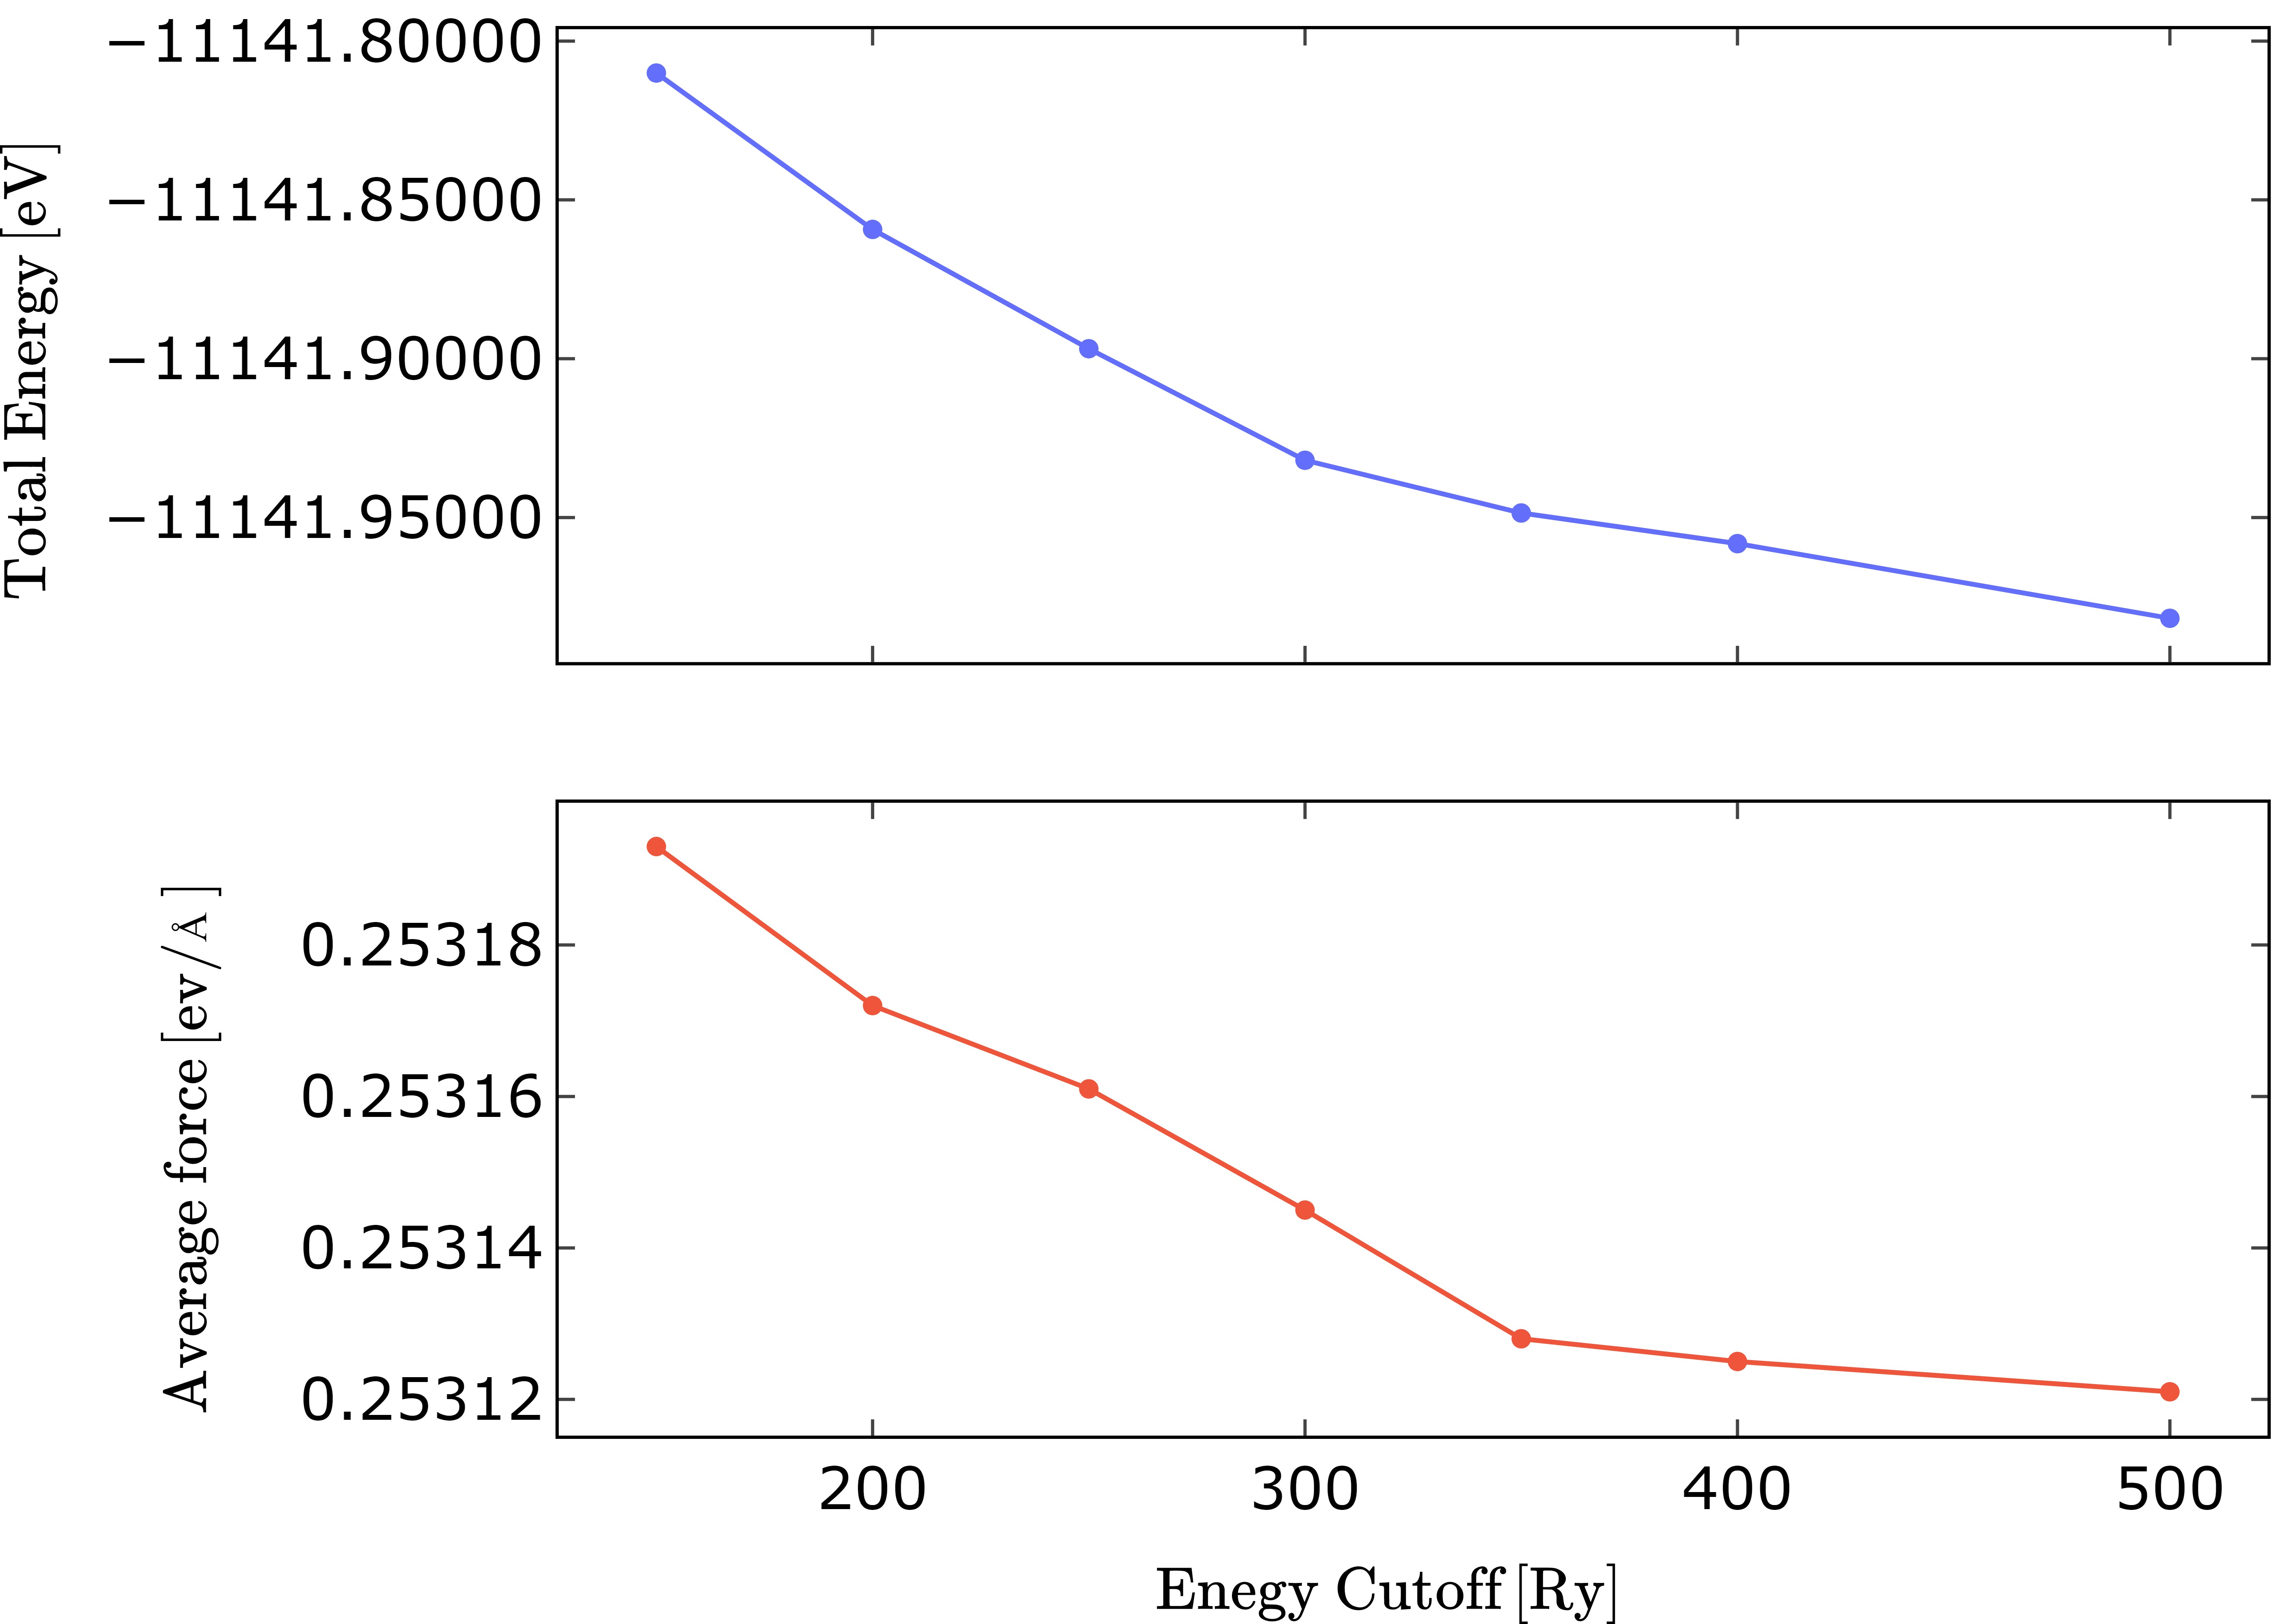
\includegraphics[width=.8\textwidth]{
      asset/cutoff_convergence.jpg
    }
  \end{center}
  \caption{Energy cutoff convergence test for the DFT training data.}
  \label{fig:dft_energy_cutoff_convergence}
\end{figure}

\begin{figure}
  \begin{center}
    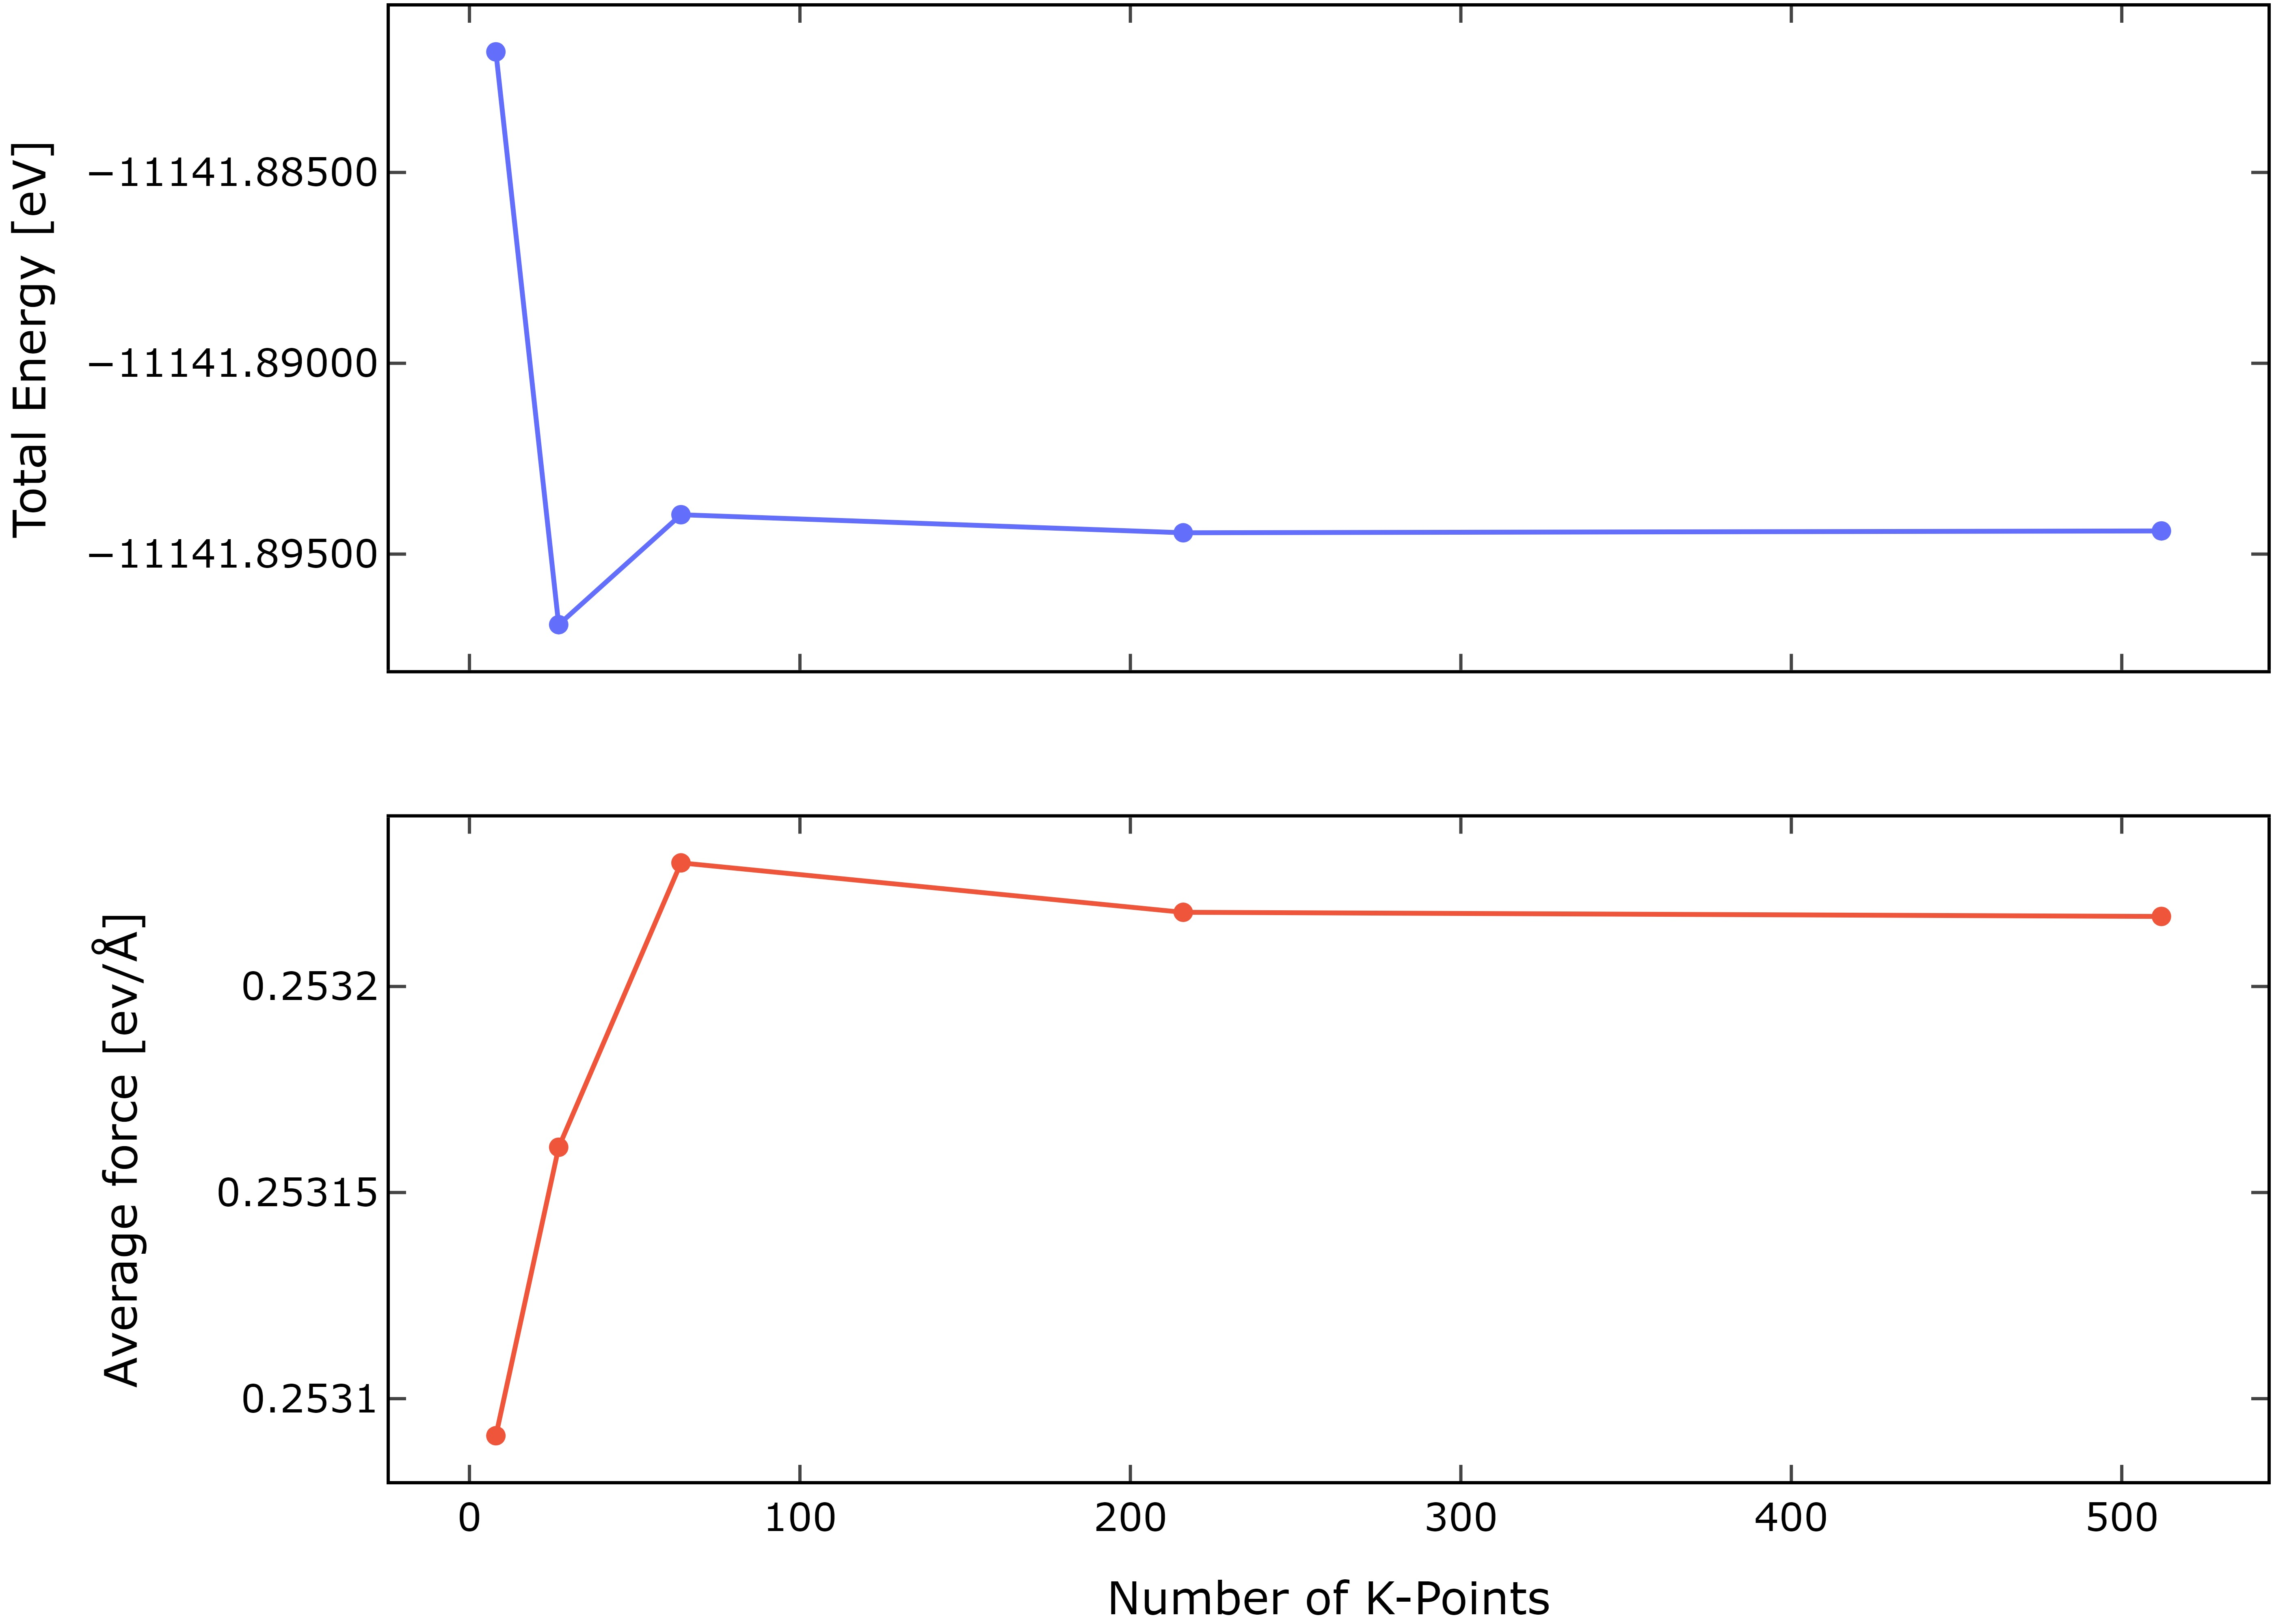
\includegraphics[width=.8\textwidth]{
      asset/kpoint_convergence.jpg
    }
  \end{center}
  \caption{K-Point convergence test for the DFT training data.}
  \label{fig:dft_kpoint_convergence}
\end{figure}

\section{Training Results}

All models were trained on dual AMD EPYC 7H12 64-Core processor machine.
Although such specs look impressive, the underlying training algorithms used
by DeepMD-kit seemd to not be optimized for CPU training and the whole process
would could probably be greatly accelerated by training on GPUs. DeepMD-kit
allows to fine-tune the training process by adjusting the runtime parameters
\texttt{OMP\_NUM\_THREADS}, \texttt{TF\_INTRA\_OP\_PARALLELISM\_THREADS}, and
\texttt{TF\_INTER\_OP\_PARALLELISM\_THREADS}. Despite running many empirical
tests to arrive at the optimal values for these parameters, the training
process did not speed up significantly. The training sessions took about
$12.01 \, \mathrm{h}$ for the larger models and about $8.29 \, \mathrm{h}$ for
the smaller models.

A typical descending learning curve was observed for models trained on the
amorphous and combined datasets. When increasing the number of descriptor
neurons from $[5, 10, 20]$ (figure
\ref{fig:amorphous_5,10,20d_20,20,20f_260222622s-learning-curves}) to
$[25, 50, 100]$ (figure
\ref{fig:amorphous_25,50,100d_20,20,20f_260222622s-learning-curves}) we don't
observe significant changes in the learning curves. On the other hand, when
increasing the number of fitting neurons from $[10, 10, 10]$
(figure \ref{fig:amorphous_10,20,40d_10,10,10f_260222622s-learning-curves}) to
$[75, 75, 75]$ (figure
\ref{fig:amorphous_10,20,40d_75,75,75f_260222622s-learning-curves}) we can
observe a very slight divergence of training error and validation error with
increasing training step. We can see from the error evaluation plot for
descriptor neurons (figure \ref{fig:descriptor_energy_error_evaluation}) that
the energy error slightly decreases with increasing number of descriptor
neurons, although this effect is negligible. The effect of increasing energy
error with increasing number of fitting neurons can also be observed in the
error evaluation plot for fitting neurons (figure
\ref{fig:fitting_energy_error_evaluation}). Both of these effects are much
more pronounced for the crystalline dataset, where data scarcity is a
significant concern. Althoug, the crystalline system should be the simplest to
model, the shortage of data plays a major role here, which can be observed in
the learning curves architectures and in the energy error evaluation plots.
The predictions for the crystalline system get outstandingly better when
increasing the number of descriptor neurons from $[5, 10, 20]$ (figure
\ref{fig:crystalline_5,10,20d_20,20,20f_260222622s-learning-curves}) to
$[25, 50, 100]$ (figure
\ref{fig:crystalline_25,50,100d_20,20,20f_260222622s-learning-curves}). This
might have several reasons. First, the higher number of descriptor neurons
make the model more flexible and more unlikely to overfit on low data volumes.
The second reason might be that the higher number of descriptor neurons allows
the model to better capture the underlying structure of the sillicon system,
since this effect is observable for the amorphous and combined systems as
well. While the number of descriptor neurons correlates positively with
inference quality, the opposite is true for the number of fitting neurons.
When increasing fitting neurons from $[10, 10, 10]$
(figure \ref{fig:crystalline_10,20,40d_10,10,10f_260222622s-learning-curves})
to $[75, 75, 75]$
(figure \ref{fig:crystalline_10,20,40d_75,75,75f_260222622s-learning-curves})
we observe the energy error increases, and the dissonance of training error
and validation error broadens. In this case, the model architecute is too
complex and underfits on the small sample of training data. We can also see
the discussed effects in the error evaluation plots for descriptor neurons
and fitting neurons (figures \ref{fig:descriptor_energy_error_evaluation} and
\ref{fig:fitting_energy_error_evaluation} respectively).


\begin{figure}
  \begin{center}
    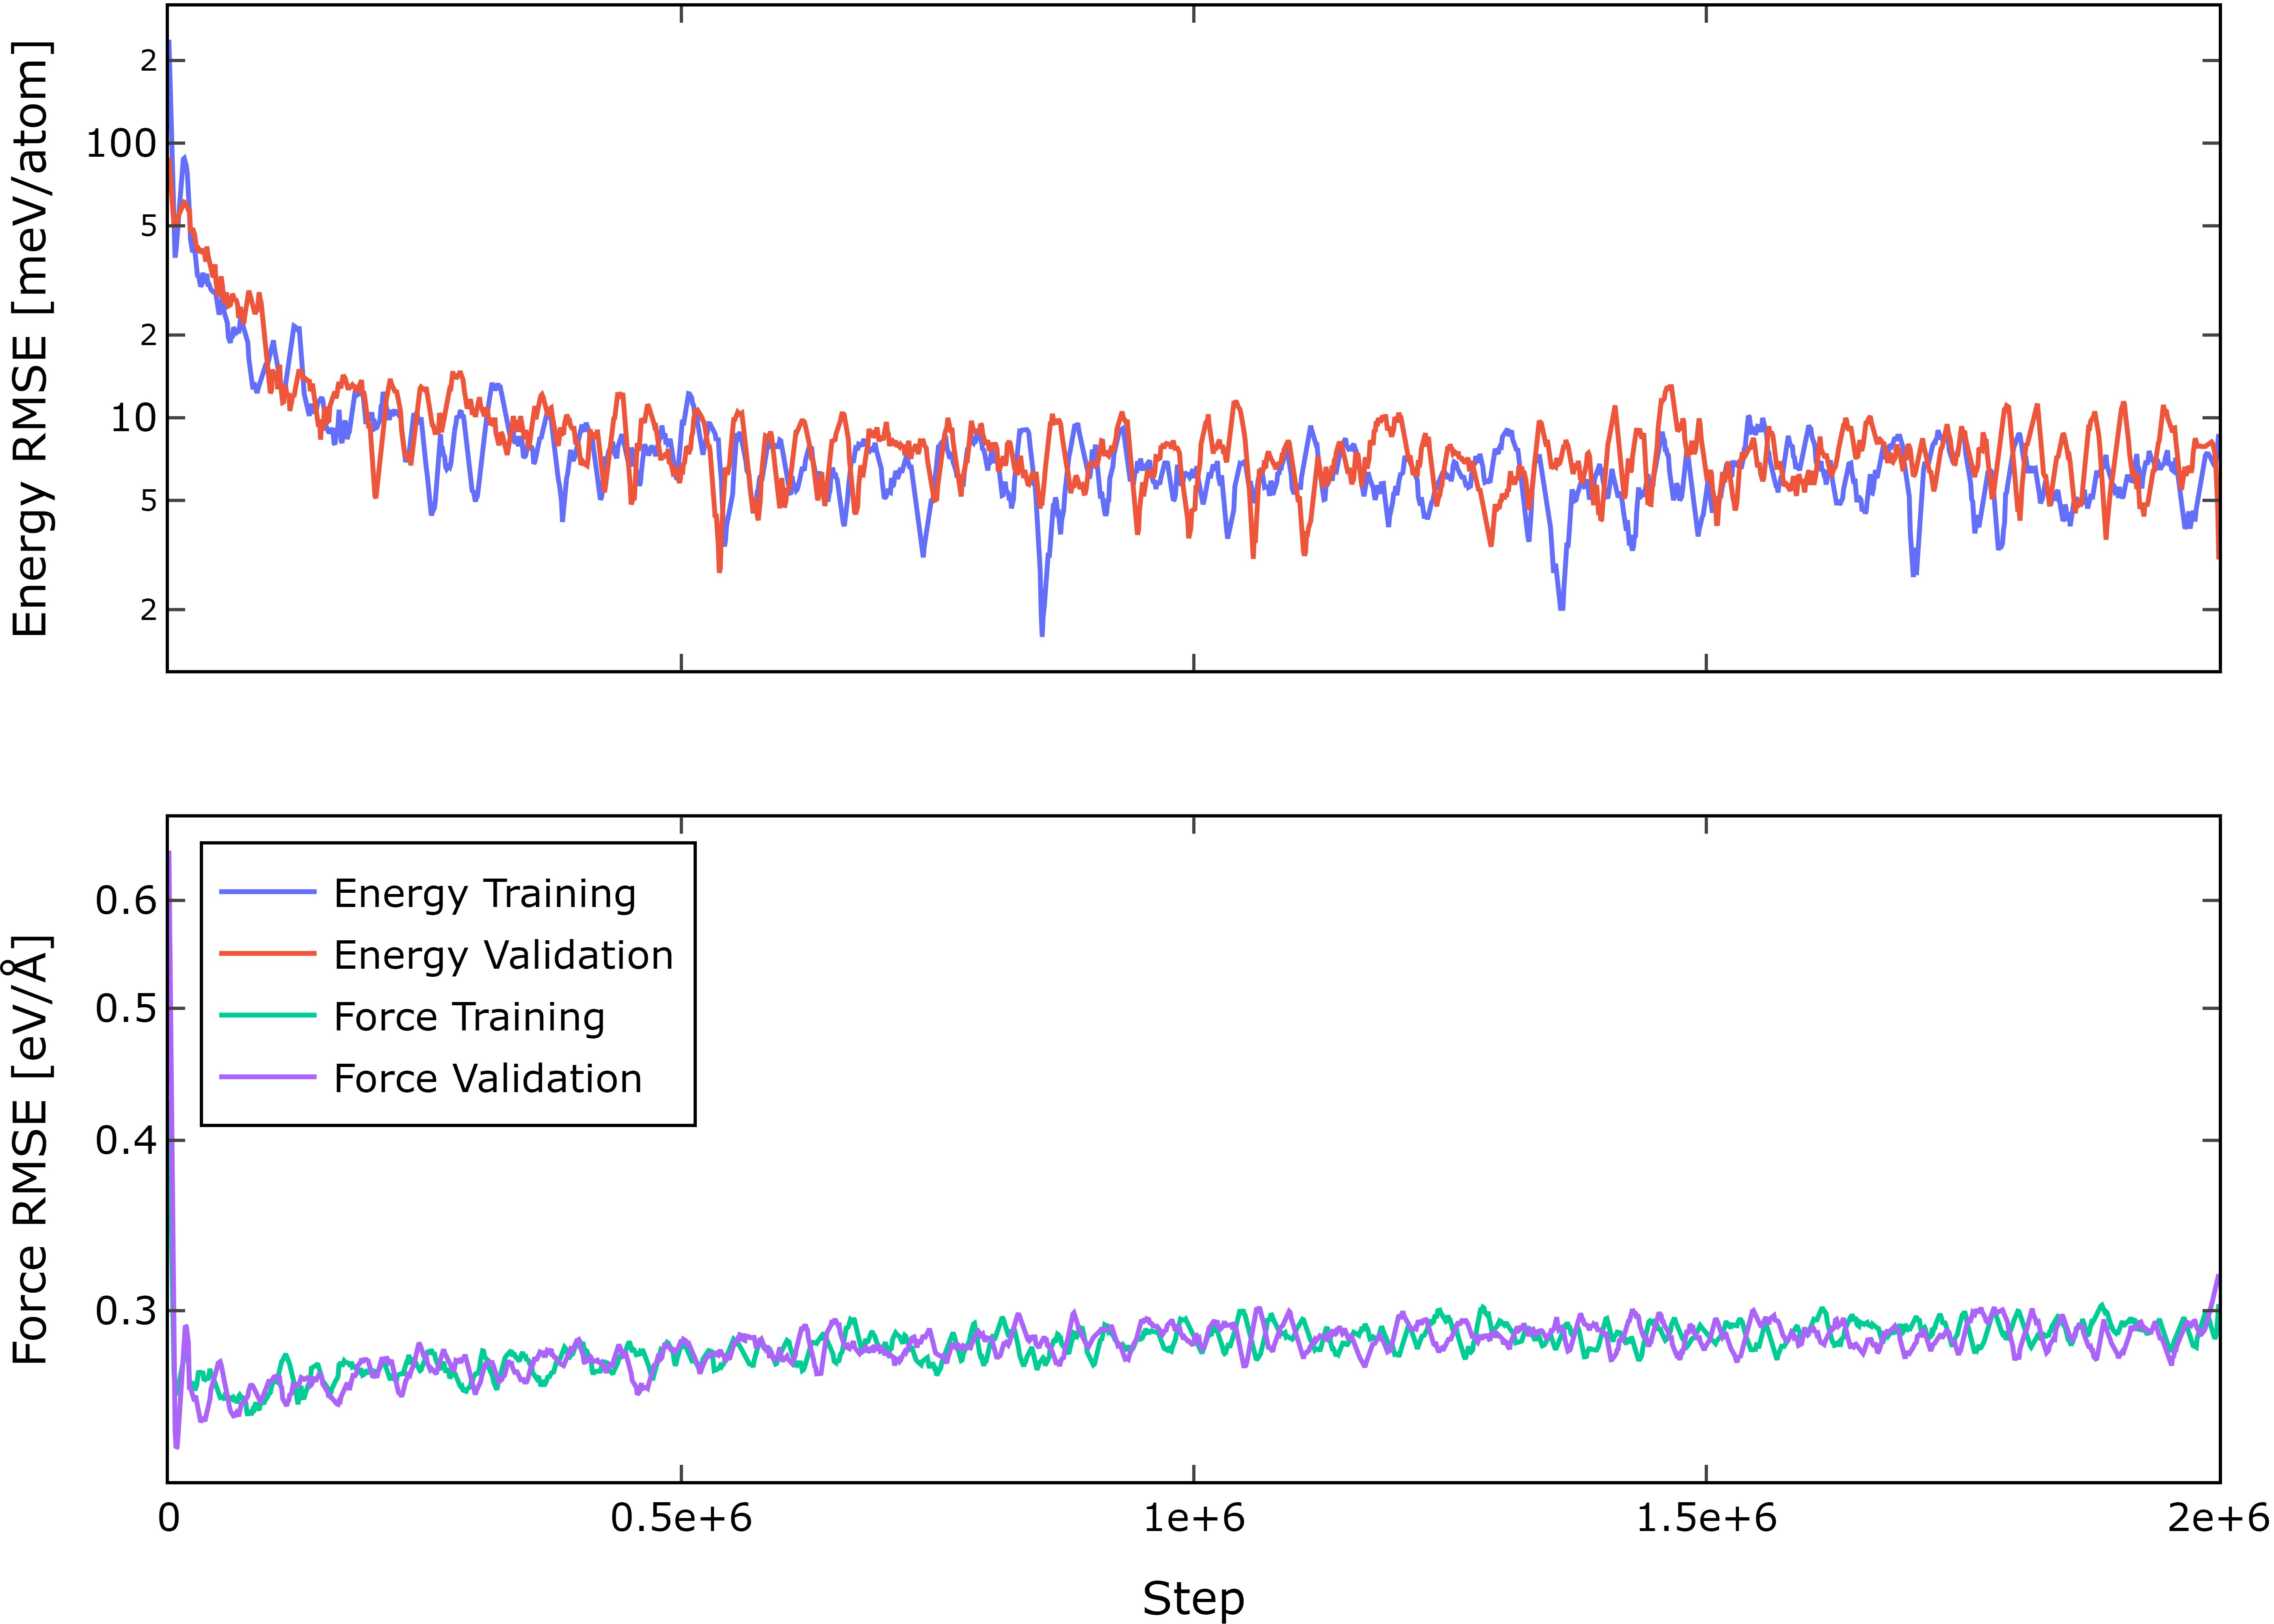
\includegraphics[width=.8\textwidth]{
      asset/amorphous_5,10,20d_20,20,20f_260222622s_energy_force_l_curve.jpg
    }
  \end{center}
  \caption{Learning curves for model \texttt{amorphous\_5,10,20d\_20,20,20f\_260222622s}.}
  \label{fig:amorphous_5,10,20d_20,20,20f_260222622s-learning-curves}
\end{figure}

\begin{figure}
  \begin{center}
    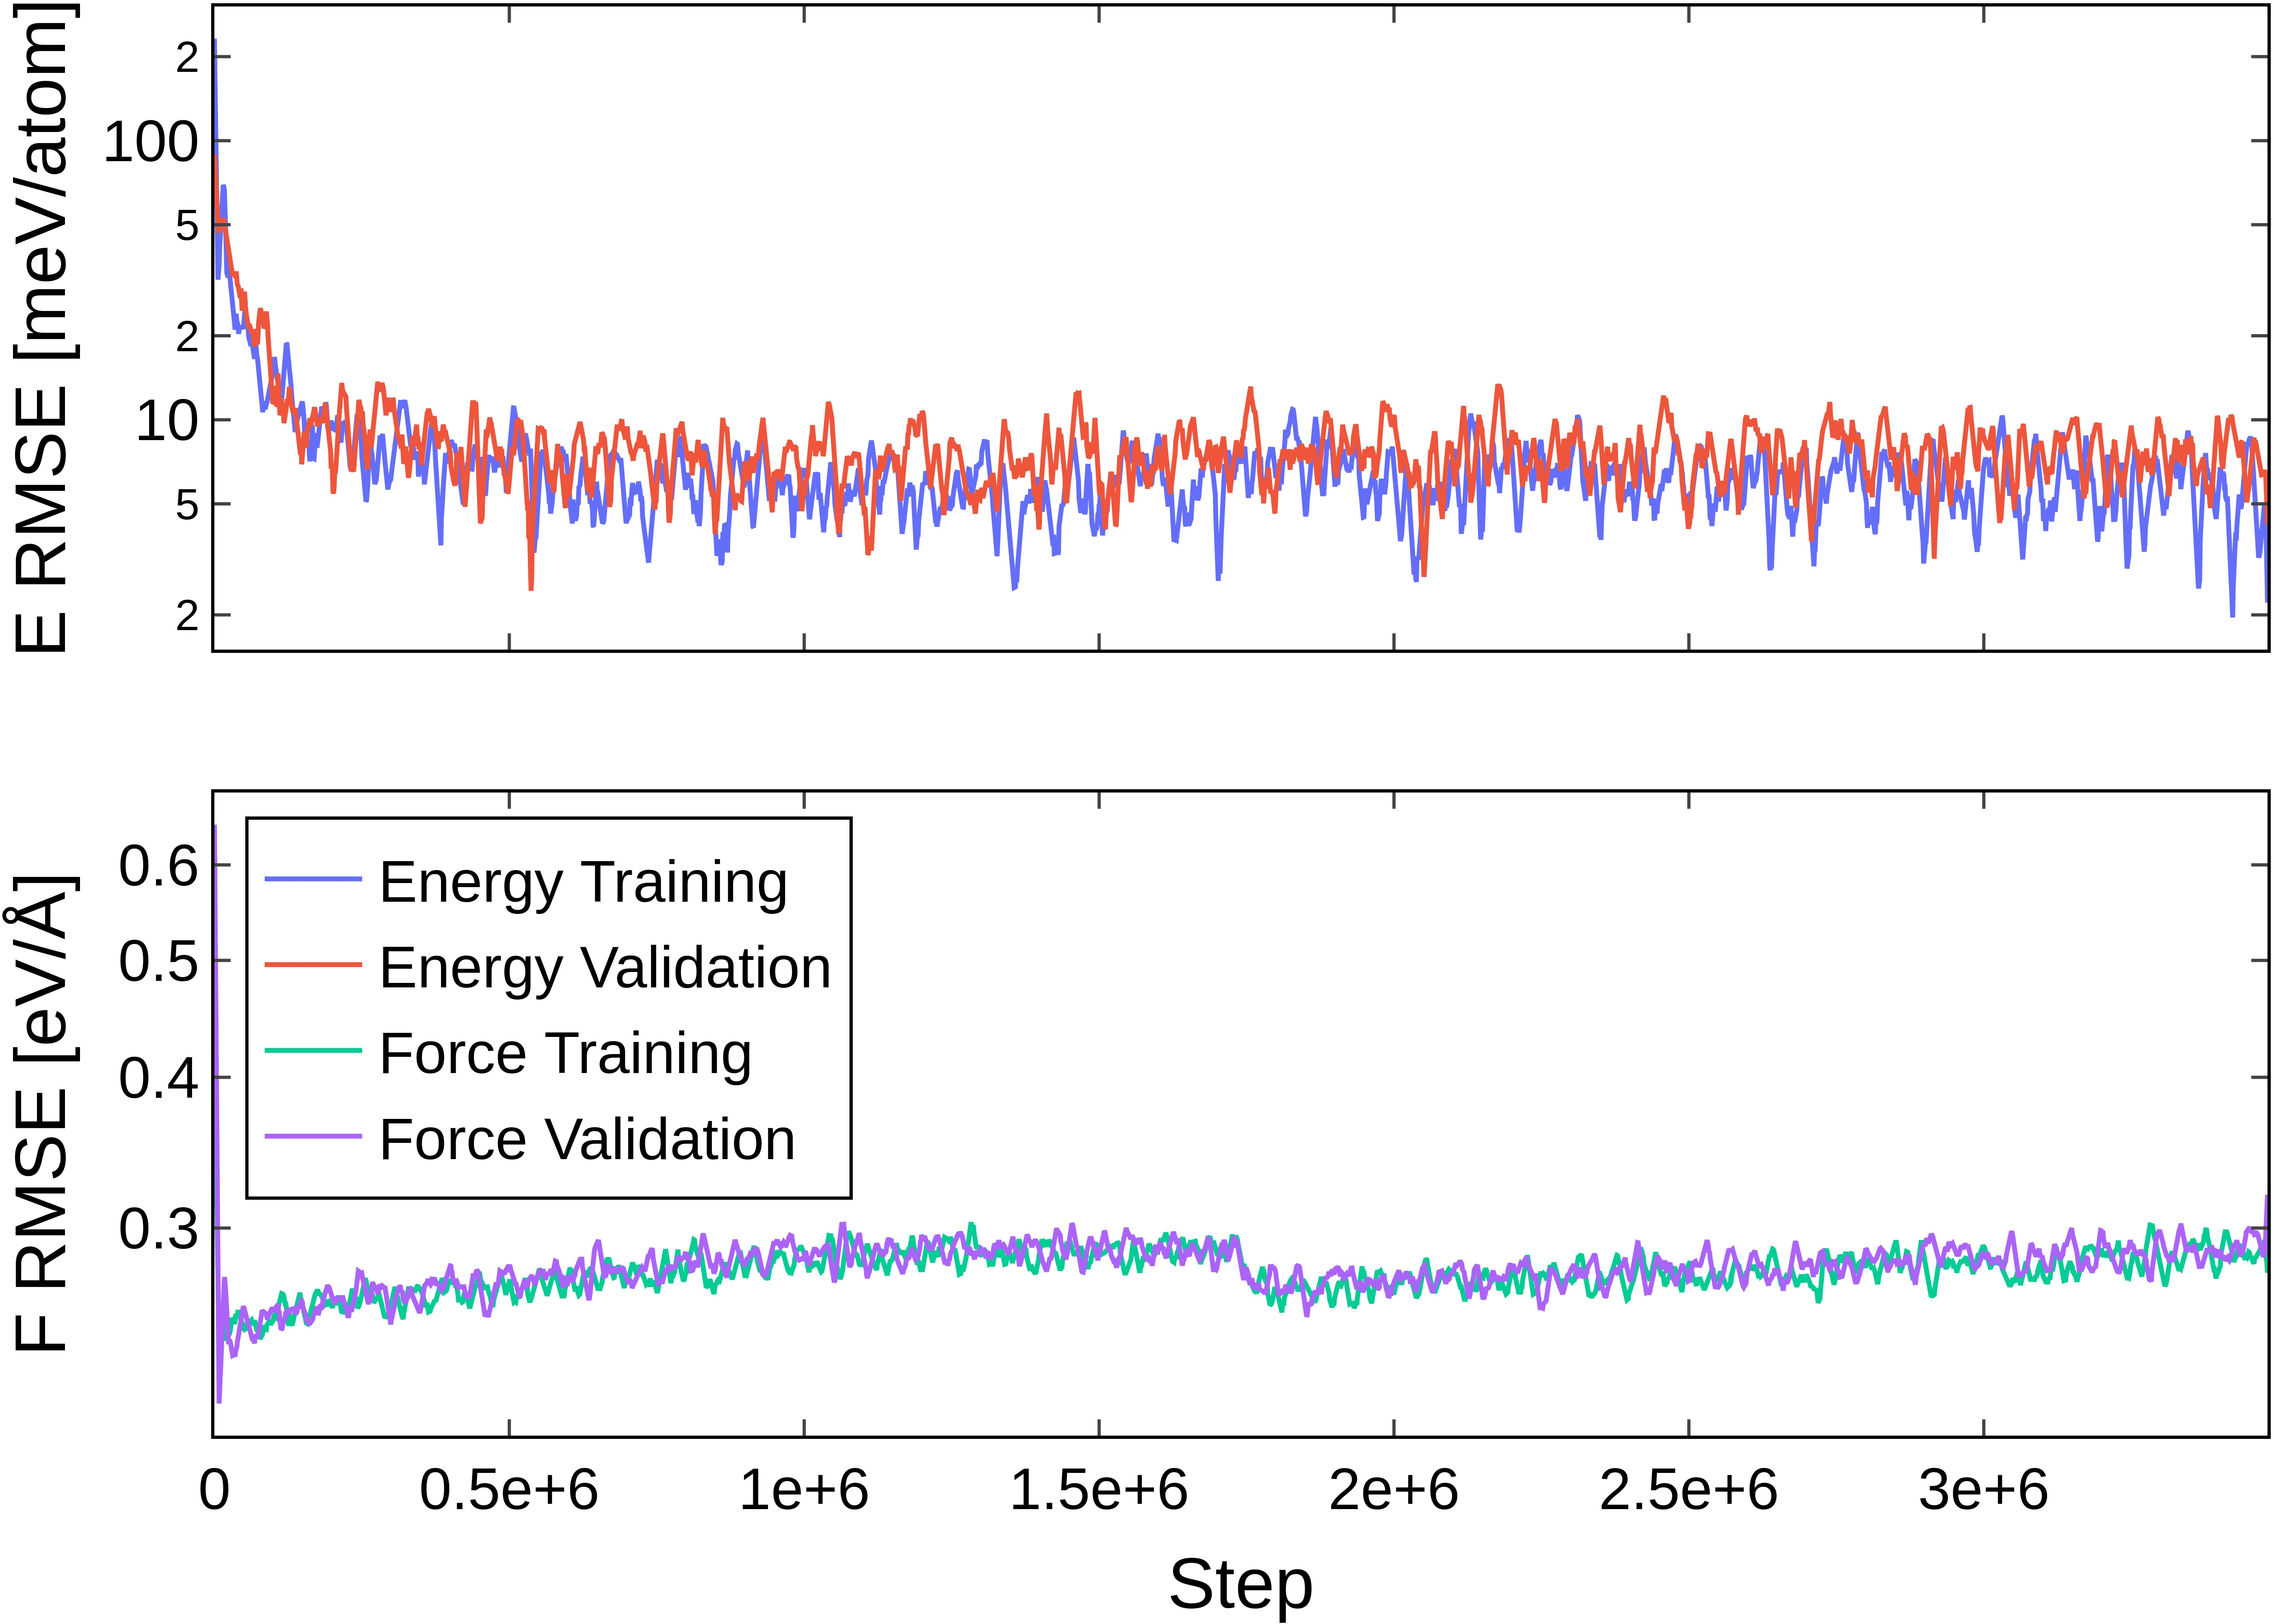
\includegraphics[width=.8\textwidth]{
      asset/amorphous_25,50,100d_20,20,20f_260222622s_energy_force_l_curve.jpg
    }
  \end{center}
  \caption{Learning curves for model \texttt{amorphous\_25,50,100d\_20,20,20f\_260222622s}.}
  \label{fig:amorphous_25,50,100d_20,20,20f_260222622s-learning-curves}
\end{figure}


\begin{figure}
  \begin{center}
    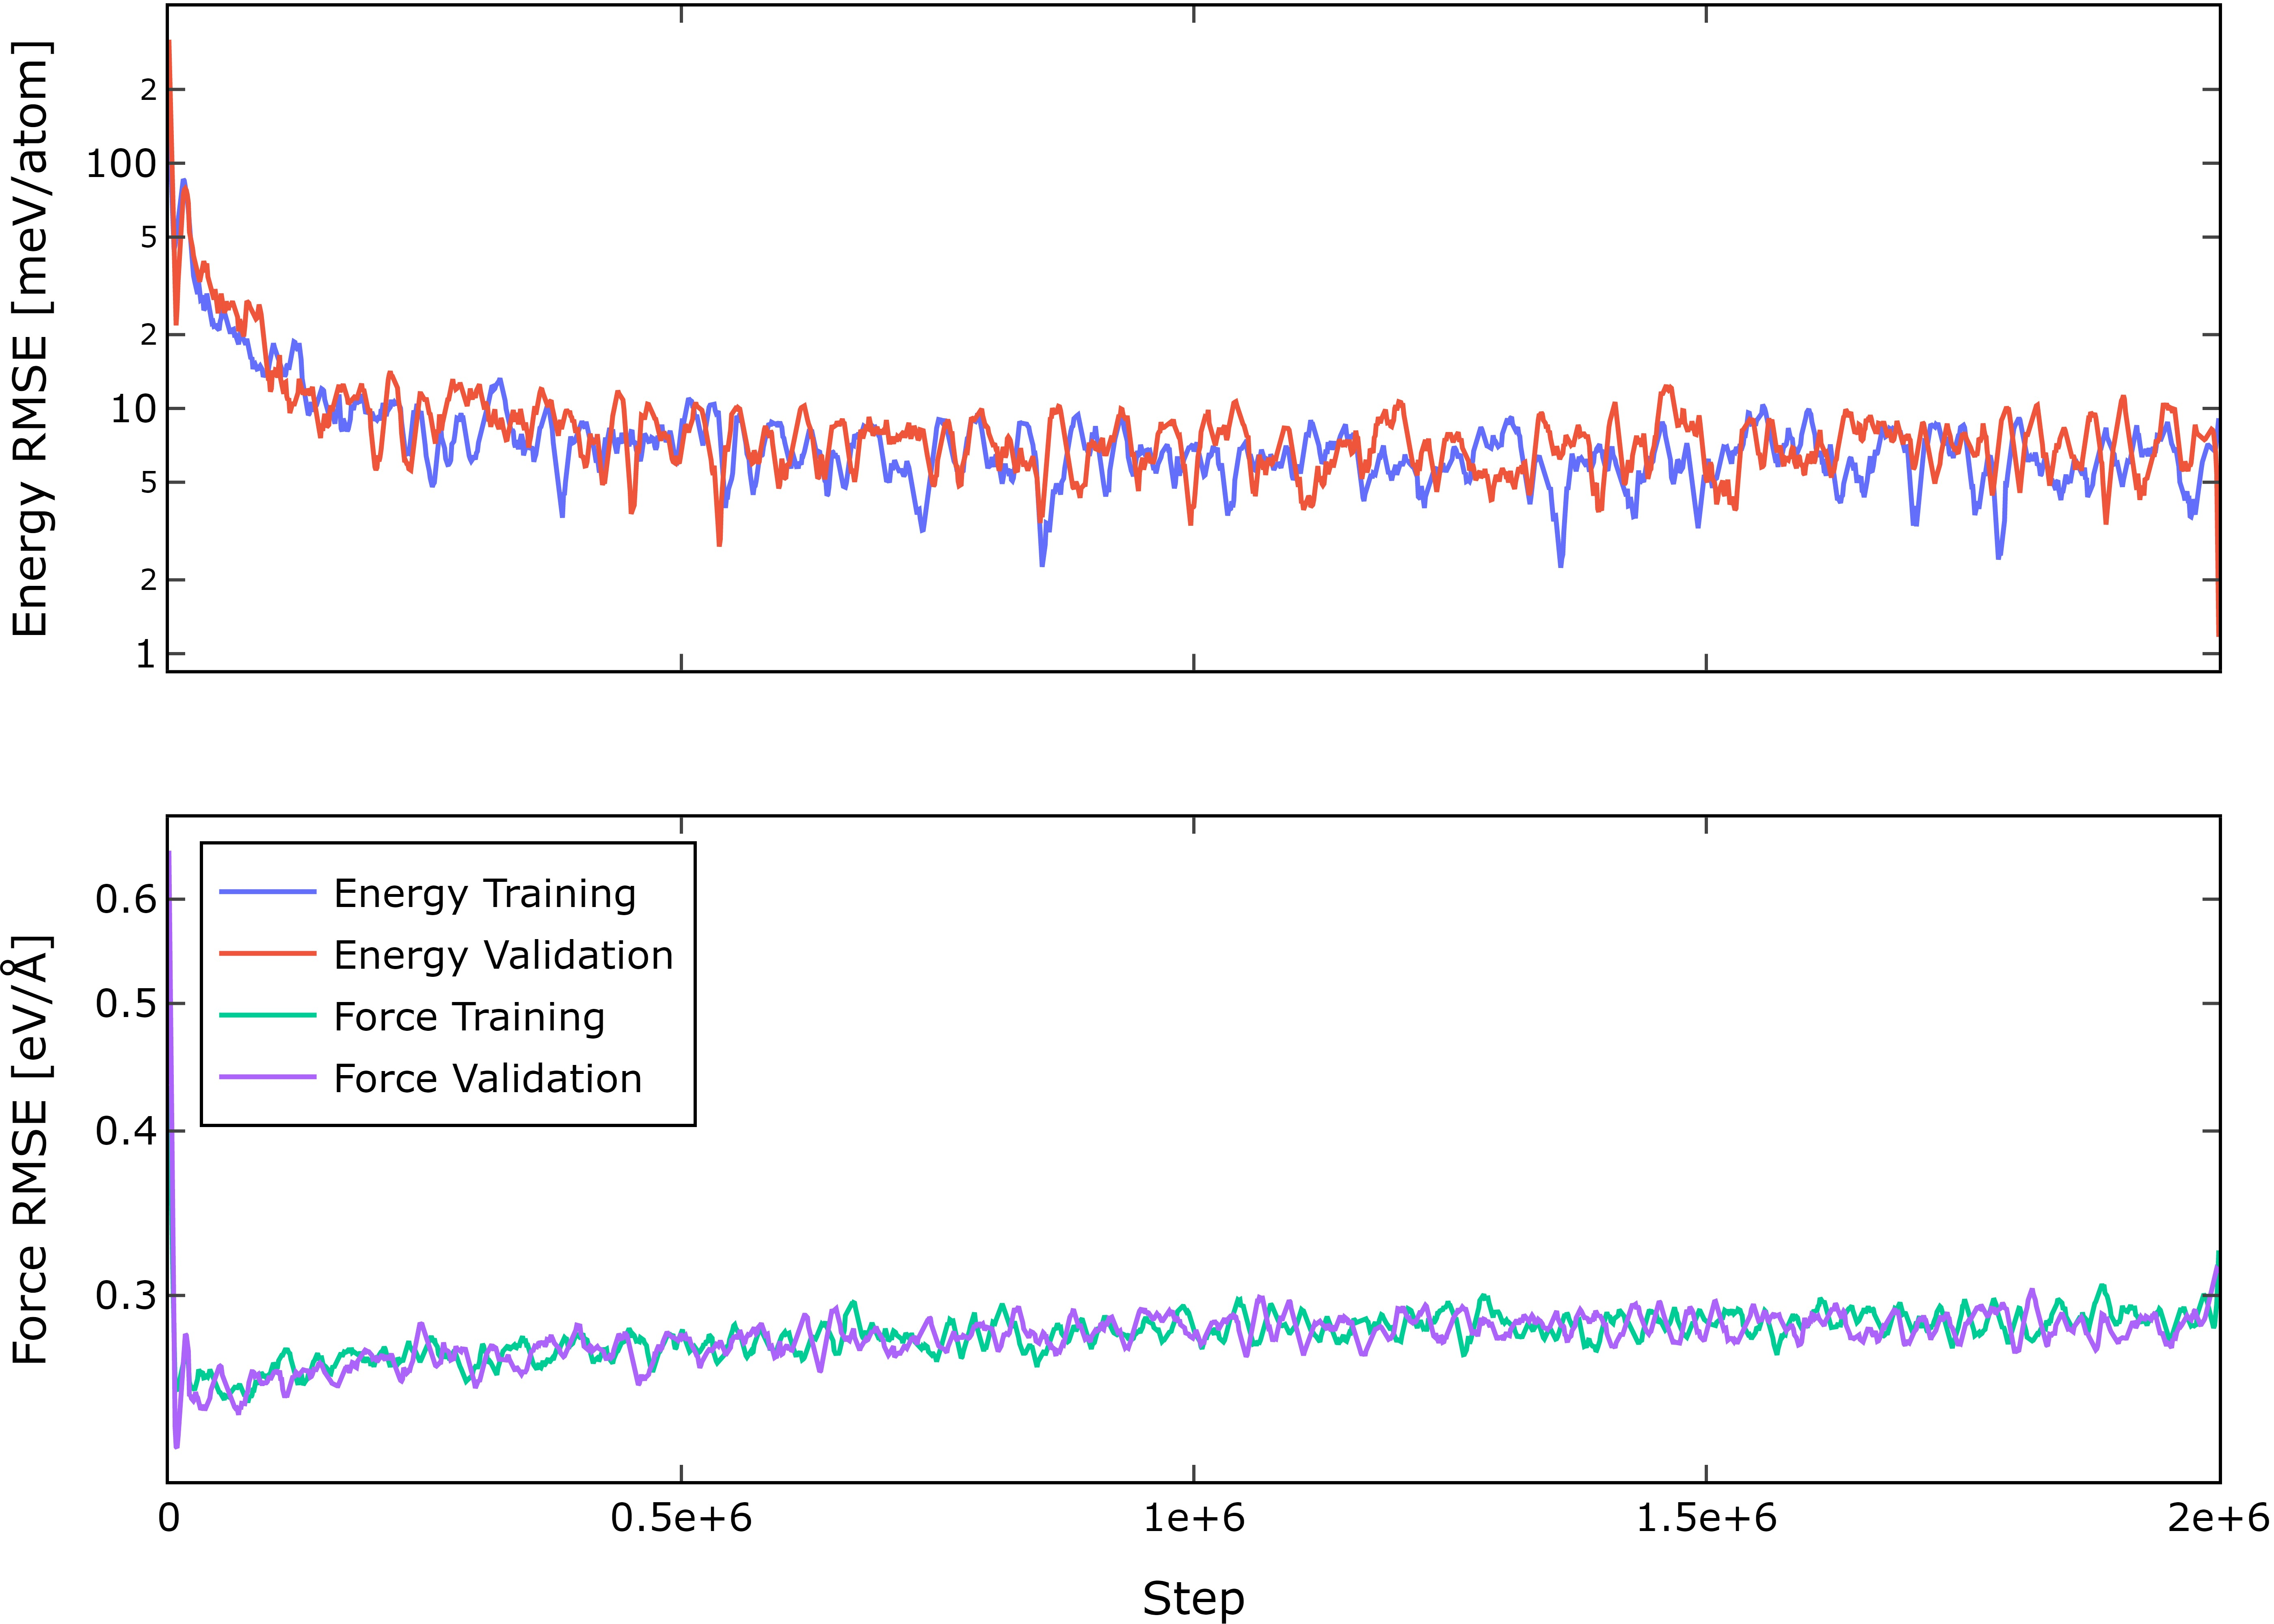
\includegraphics[width=.8\textwidth]{
      asset/amorphous_10,20,40d_10,10,10f_260222622s_energy_force_l_curve.jpg
    }
  \end{center}
  \caption{Learning curves for model \texttt{amorphous\_10,20,40d\_10,10,10f\_260222622s}.}
  \label{fig:amorphous_10,20,40d_10,10,10f_260222622s-learning-curves}
\end{figure}

\begin{figure}
  \begin{center}
    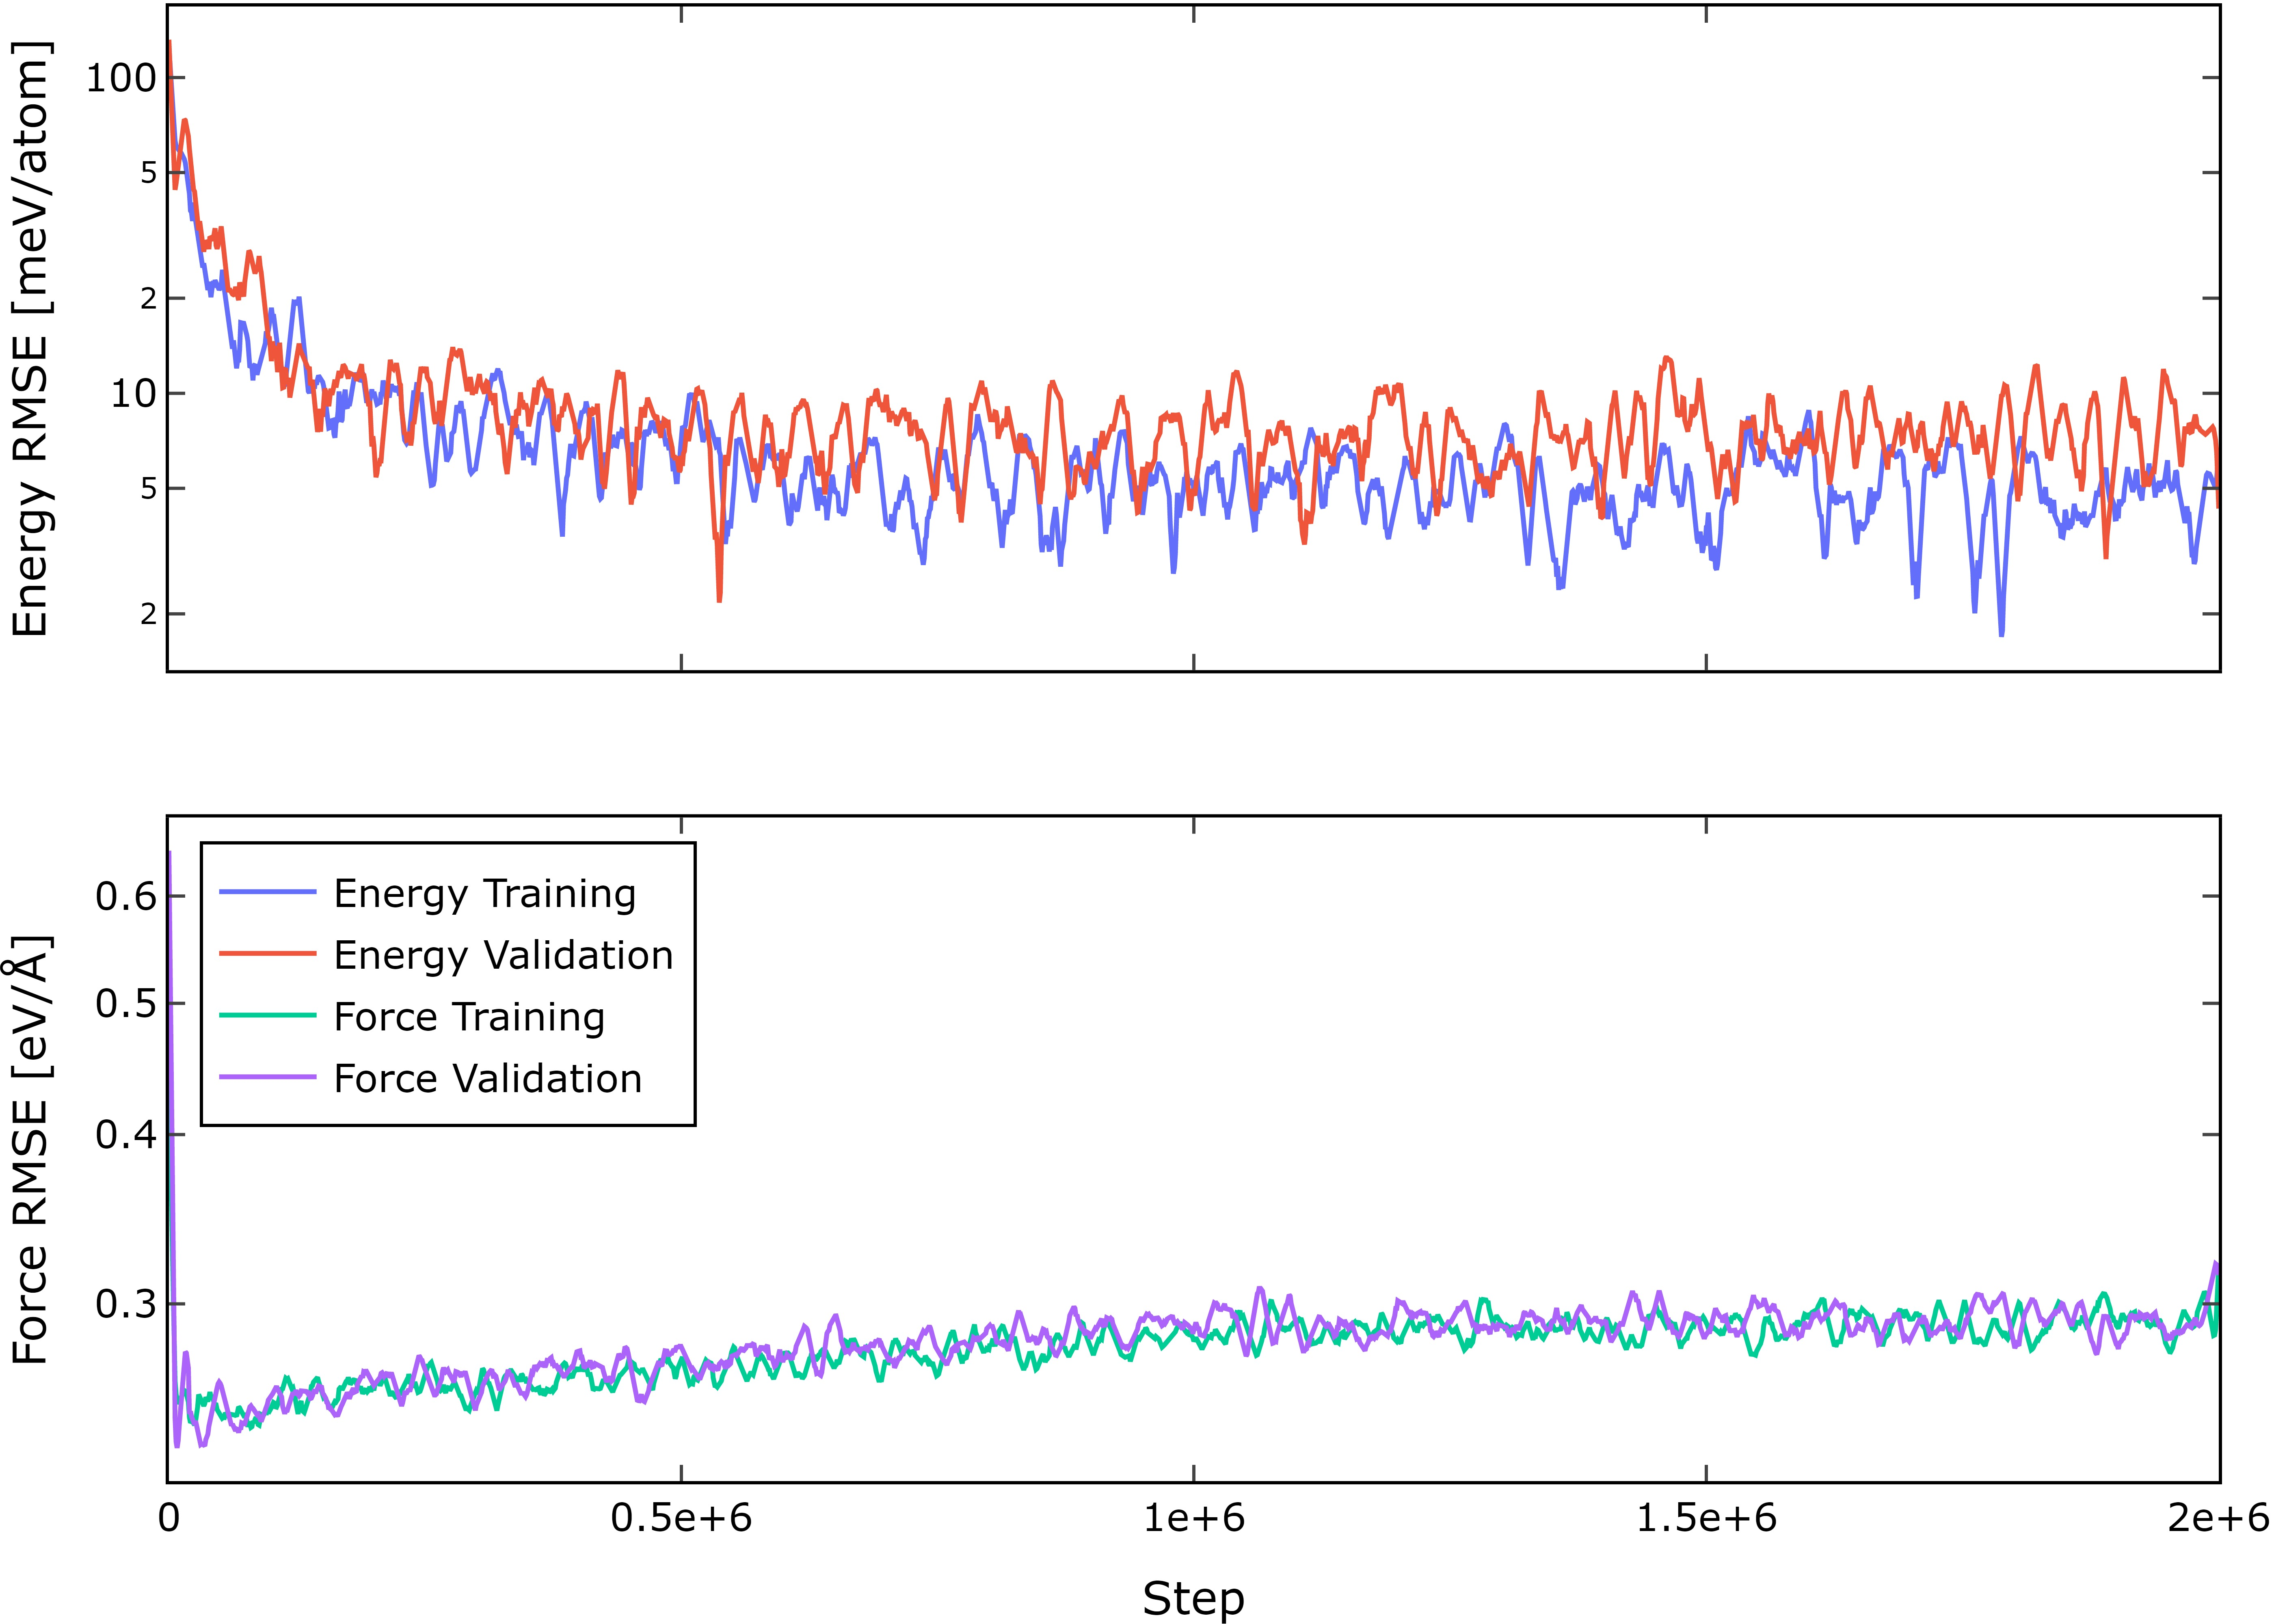
\includegraphics[width=.8\textwidth]{
      asset/amorphous_10,20,40d_75,75,75f_260222622s_energy_force_l_curve.jpg
    }
  \end{center}
  \caption{Learning curves for model \texttt{amorphous\_10,20,40d\_75,75,75f\_260222622s}.}
  \label{fig:amorphous_10,20,40d_75,75,75f_260222622s-learning-curves}
\end{figure}

\begin{figure}
  \begin{center}
    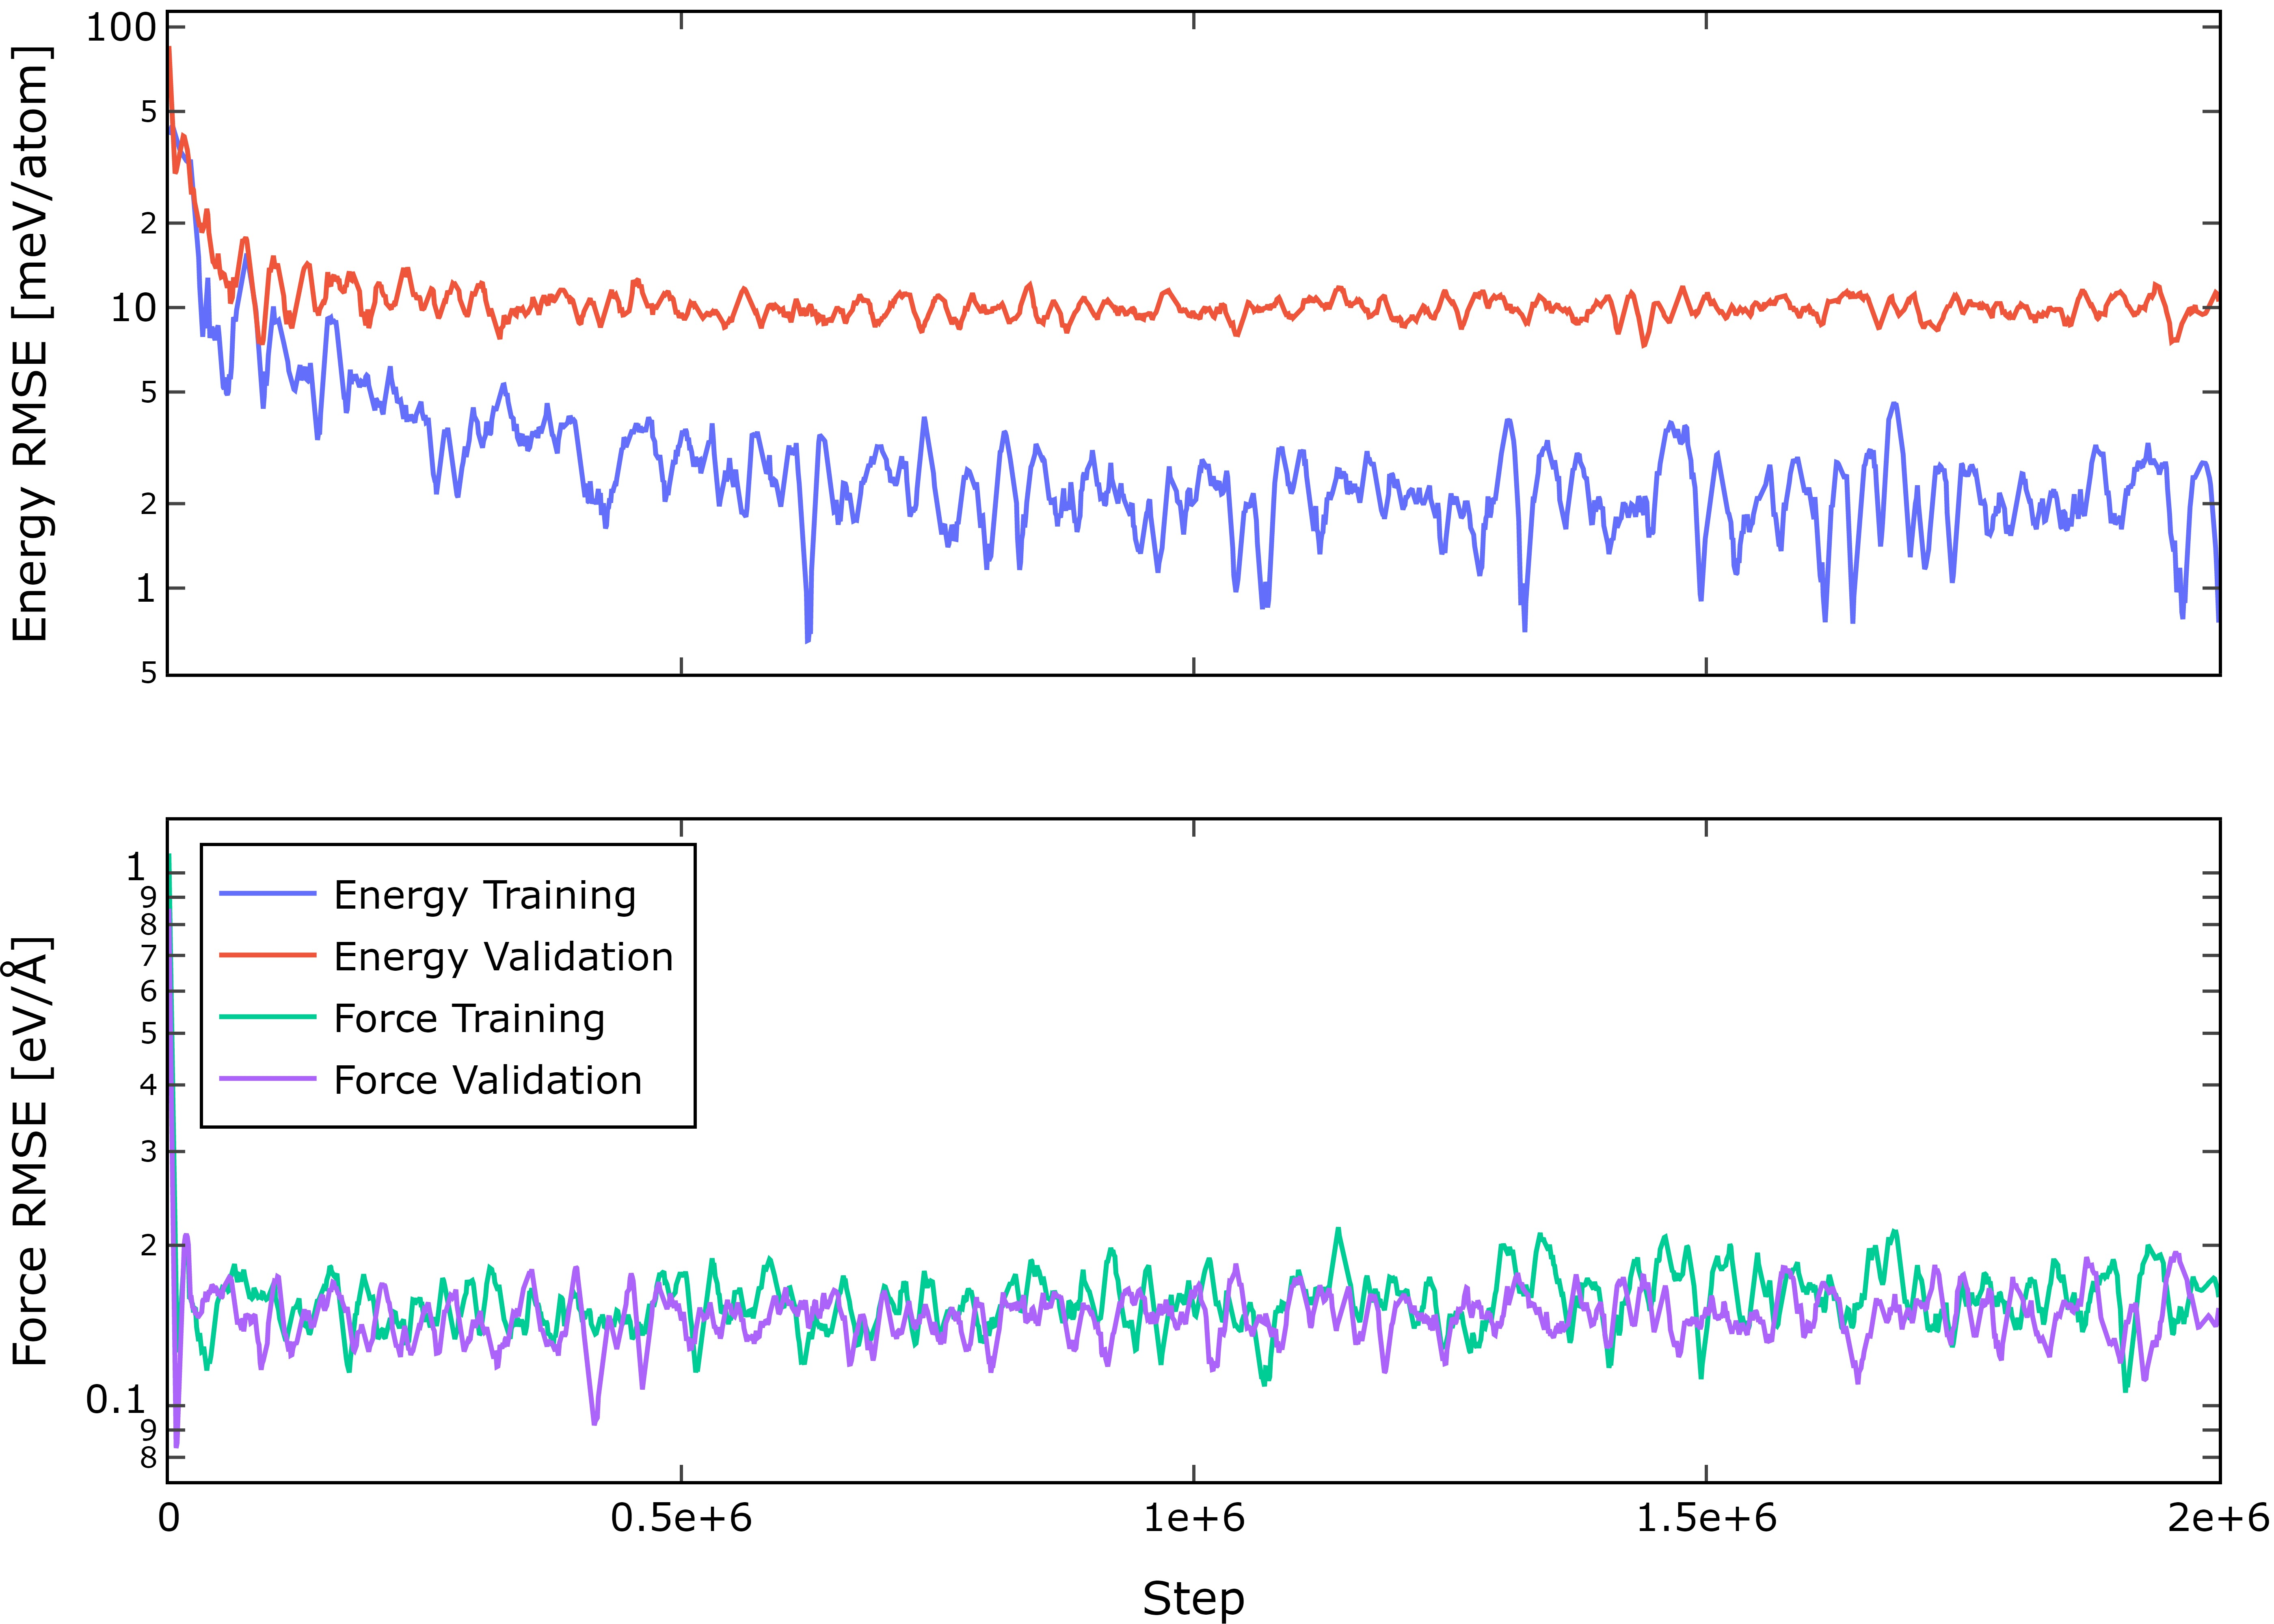
\includegraphics[width=.8\textwidth]{
      asset/crystalline_5,10,20d_20,20,20f_260222622s_energy_force_l_curve.jpg
    }
  \end{center}
  \caption{Learning curves for model \texttt{crystalline\_5,10,20d\_20,20,20f\_260222622s}.}
  \label{fig:crystalline_5,10,20d_20,20,20f_260222622s-learning-curves}
\end{figure}

\begin{figure}
  \begin{center}
    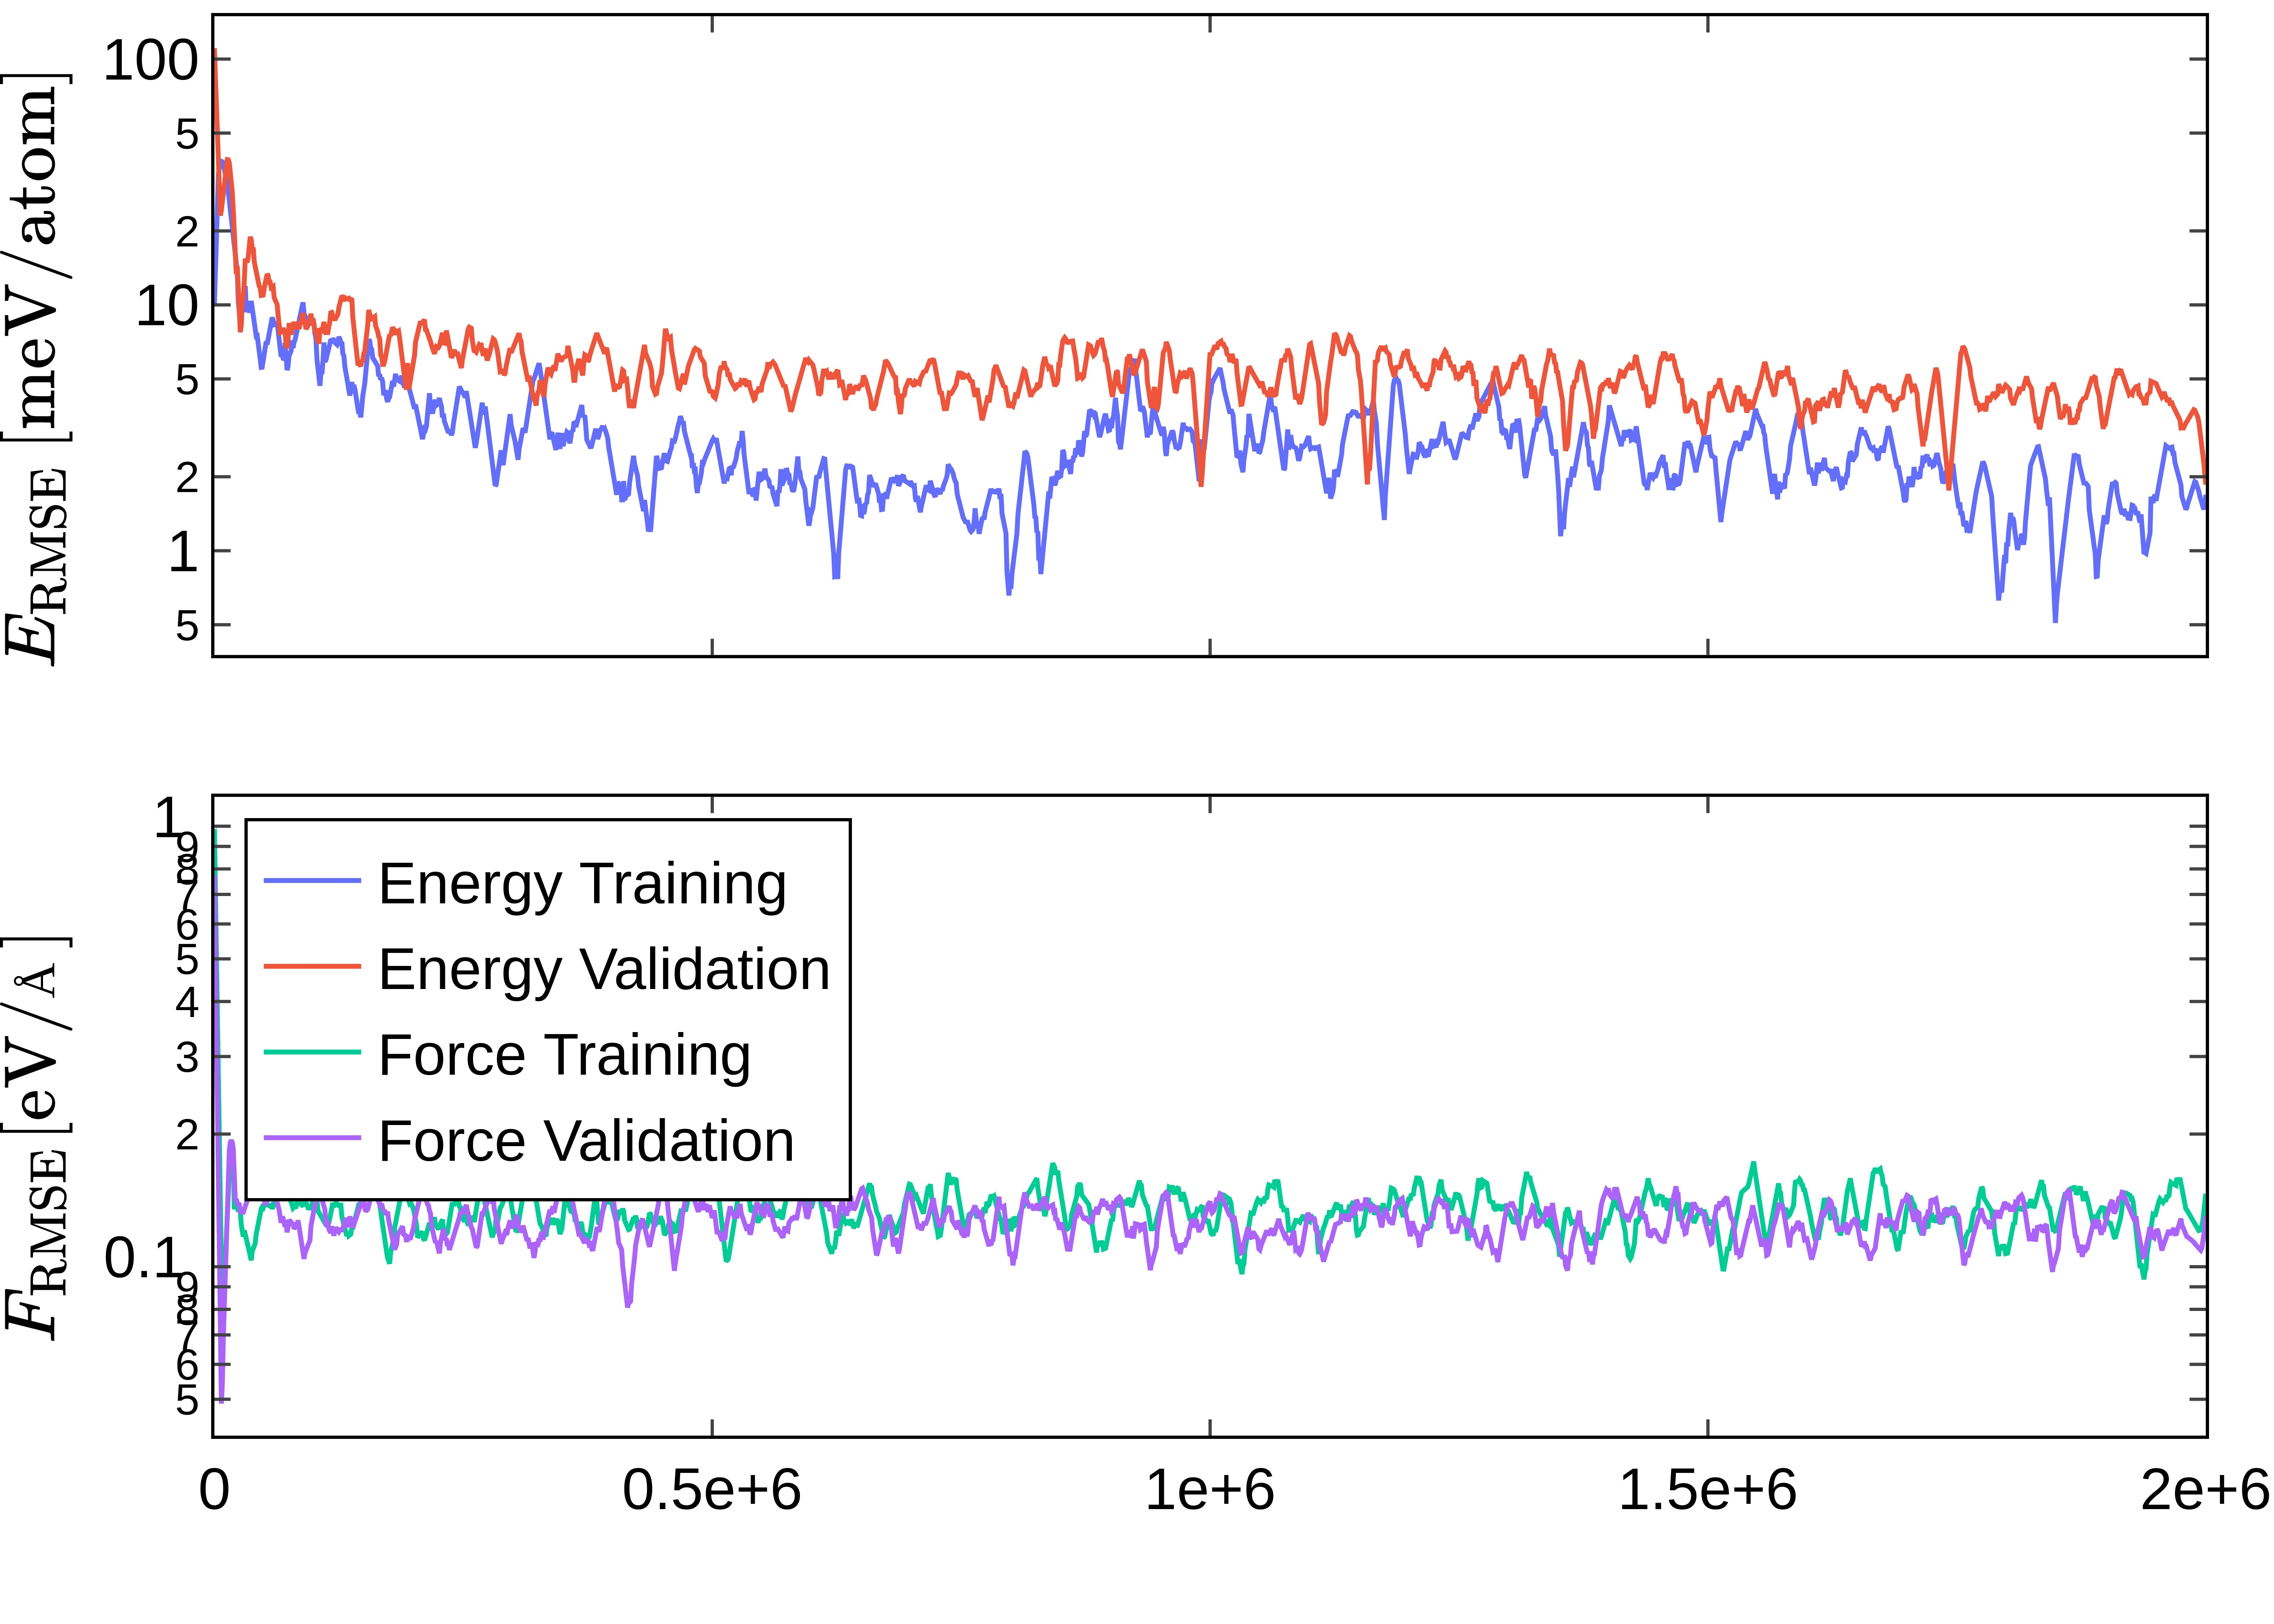
\includegraphics[width=.8\textwidth]{
      asset/crystalline_25,50,100d_20,20,20f_260222622s_energy_force_l_curve.jpg
    }
  \end{center}
  \caption{Learning curves for model \texttt{crystalline\_25,50,100d\_20,20,20f\_260222622s}.}
  \label{fig:crystalline_25,50,100d_20,20,20f_260222622s-learning-curves}
\end{figure}

\begin{figure}
  \begin{center}
    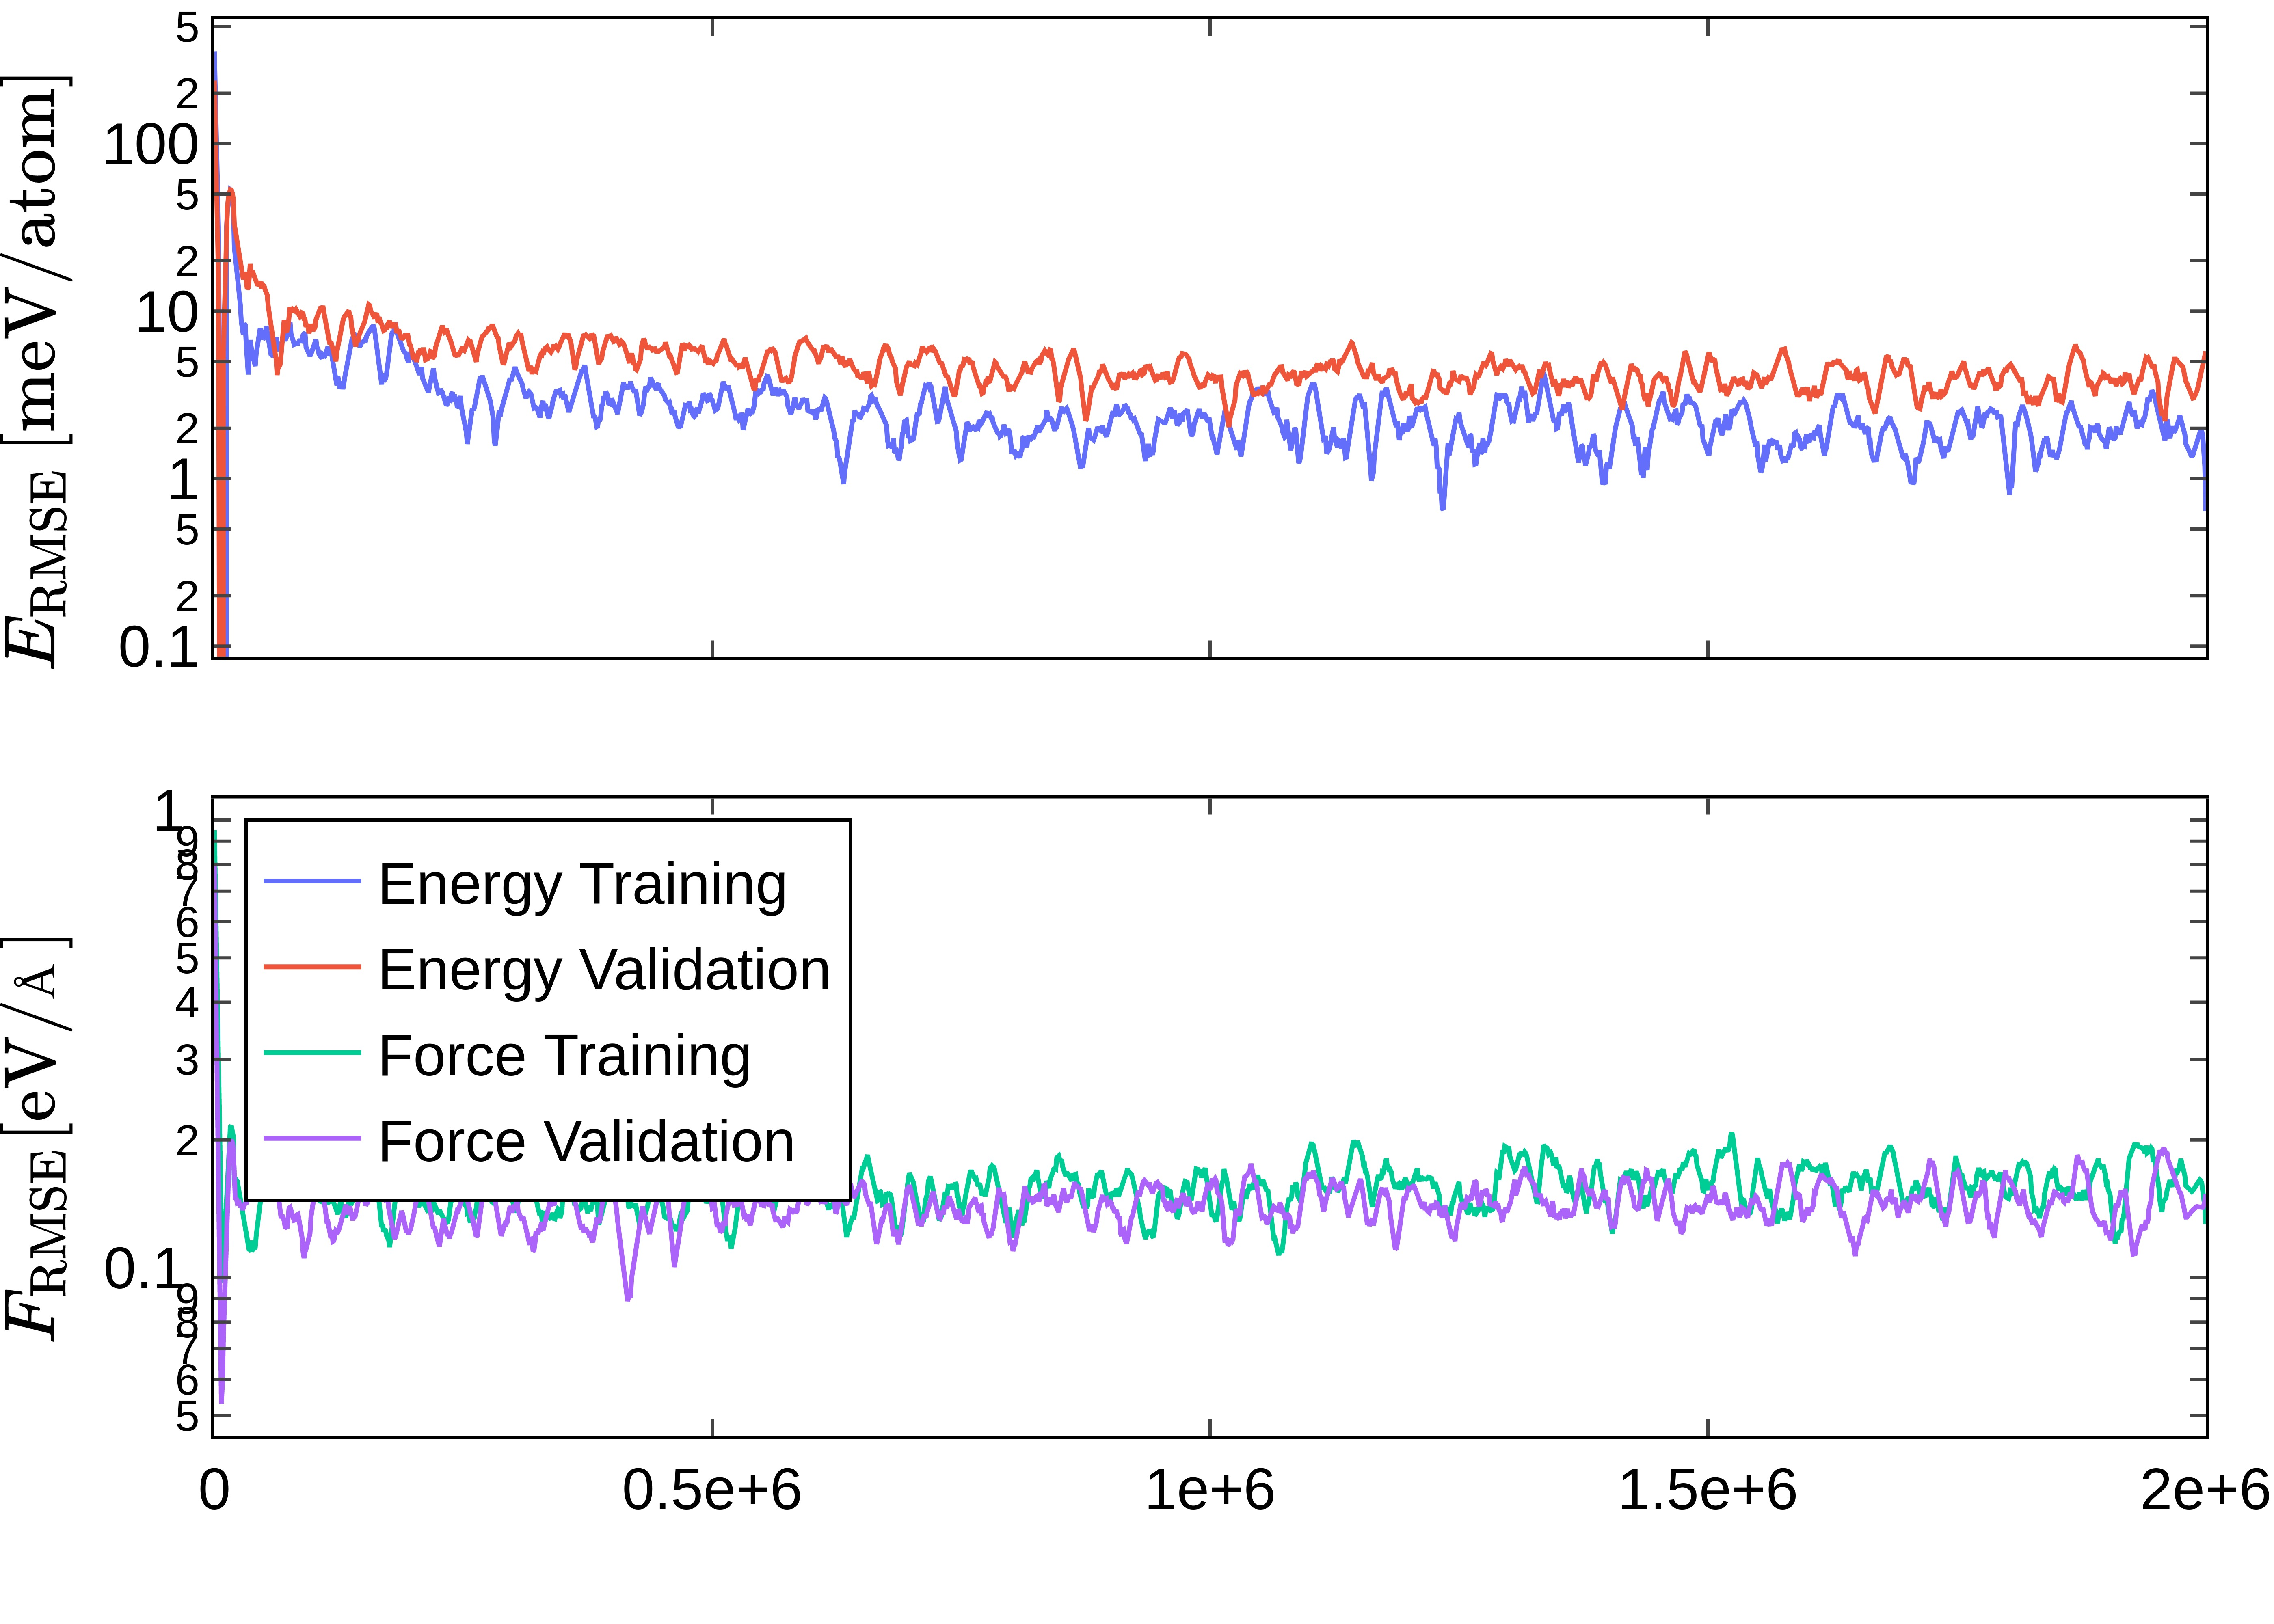
\includegraphics[width=.8\textwidth]{
      asset/crystalline_10,20,40d_10,10,10f_260222622s_energy_force_l_curve.jpg
    }
  \end{center}
  \caption{Learning curves for model \texttt{crystalline\_10,20,40d\_10,10,10f\_260222622s}.}
  \label{fig:crystalline_10,20,40d_10,10,10f_260222622s-learning-curves}
\end{figure}

\begin{figure}
  \begin{center}
    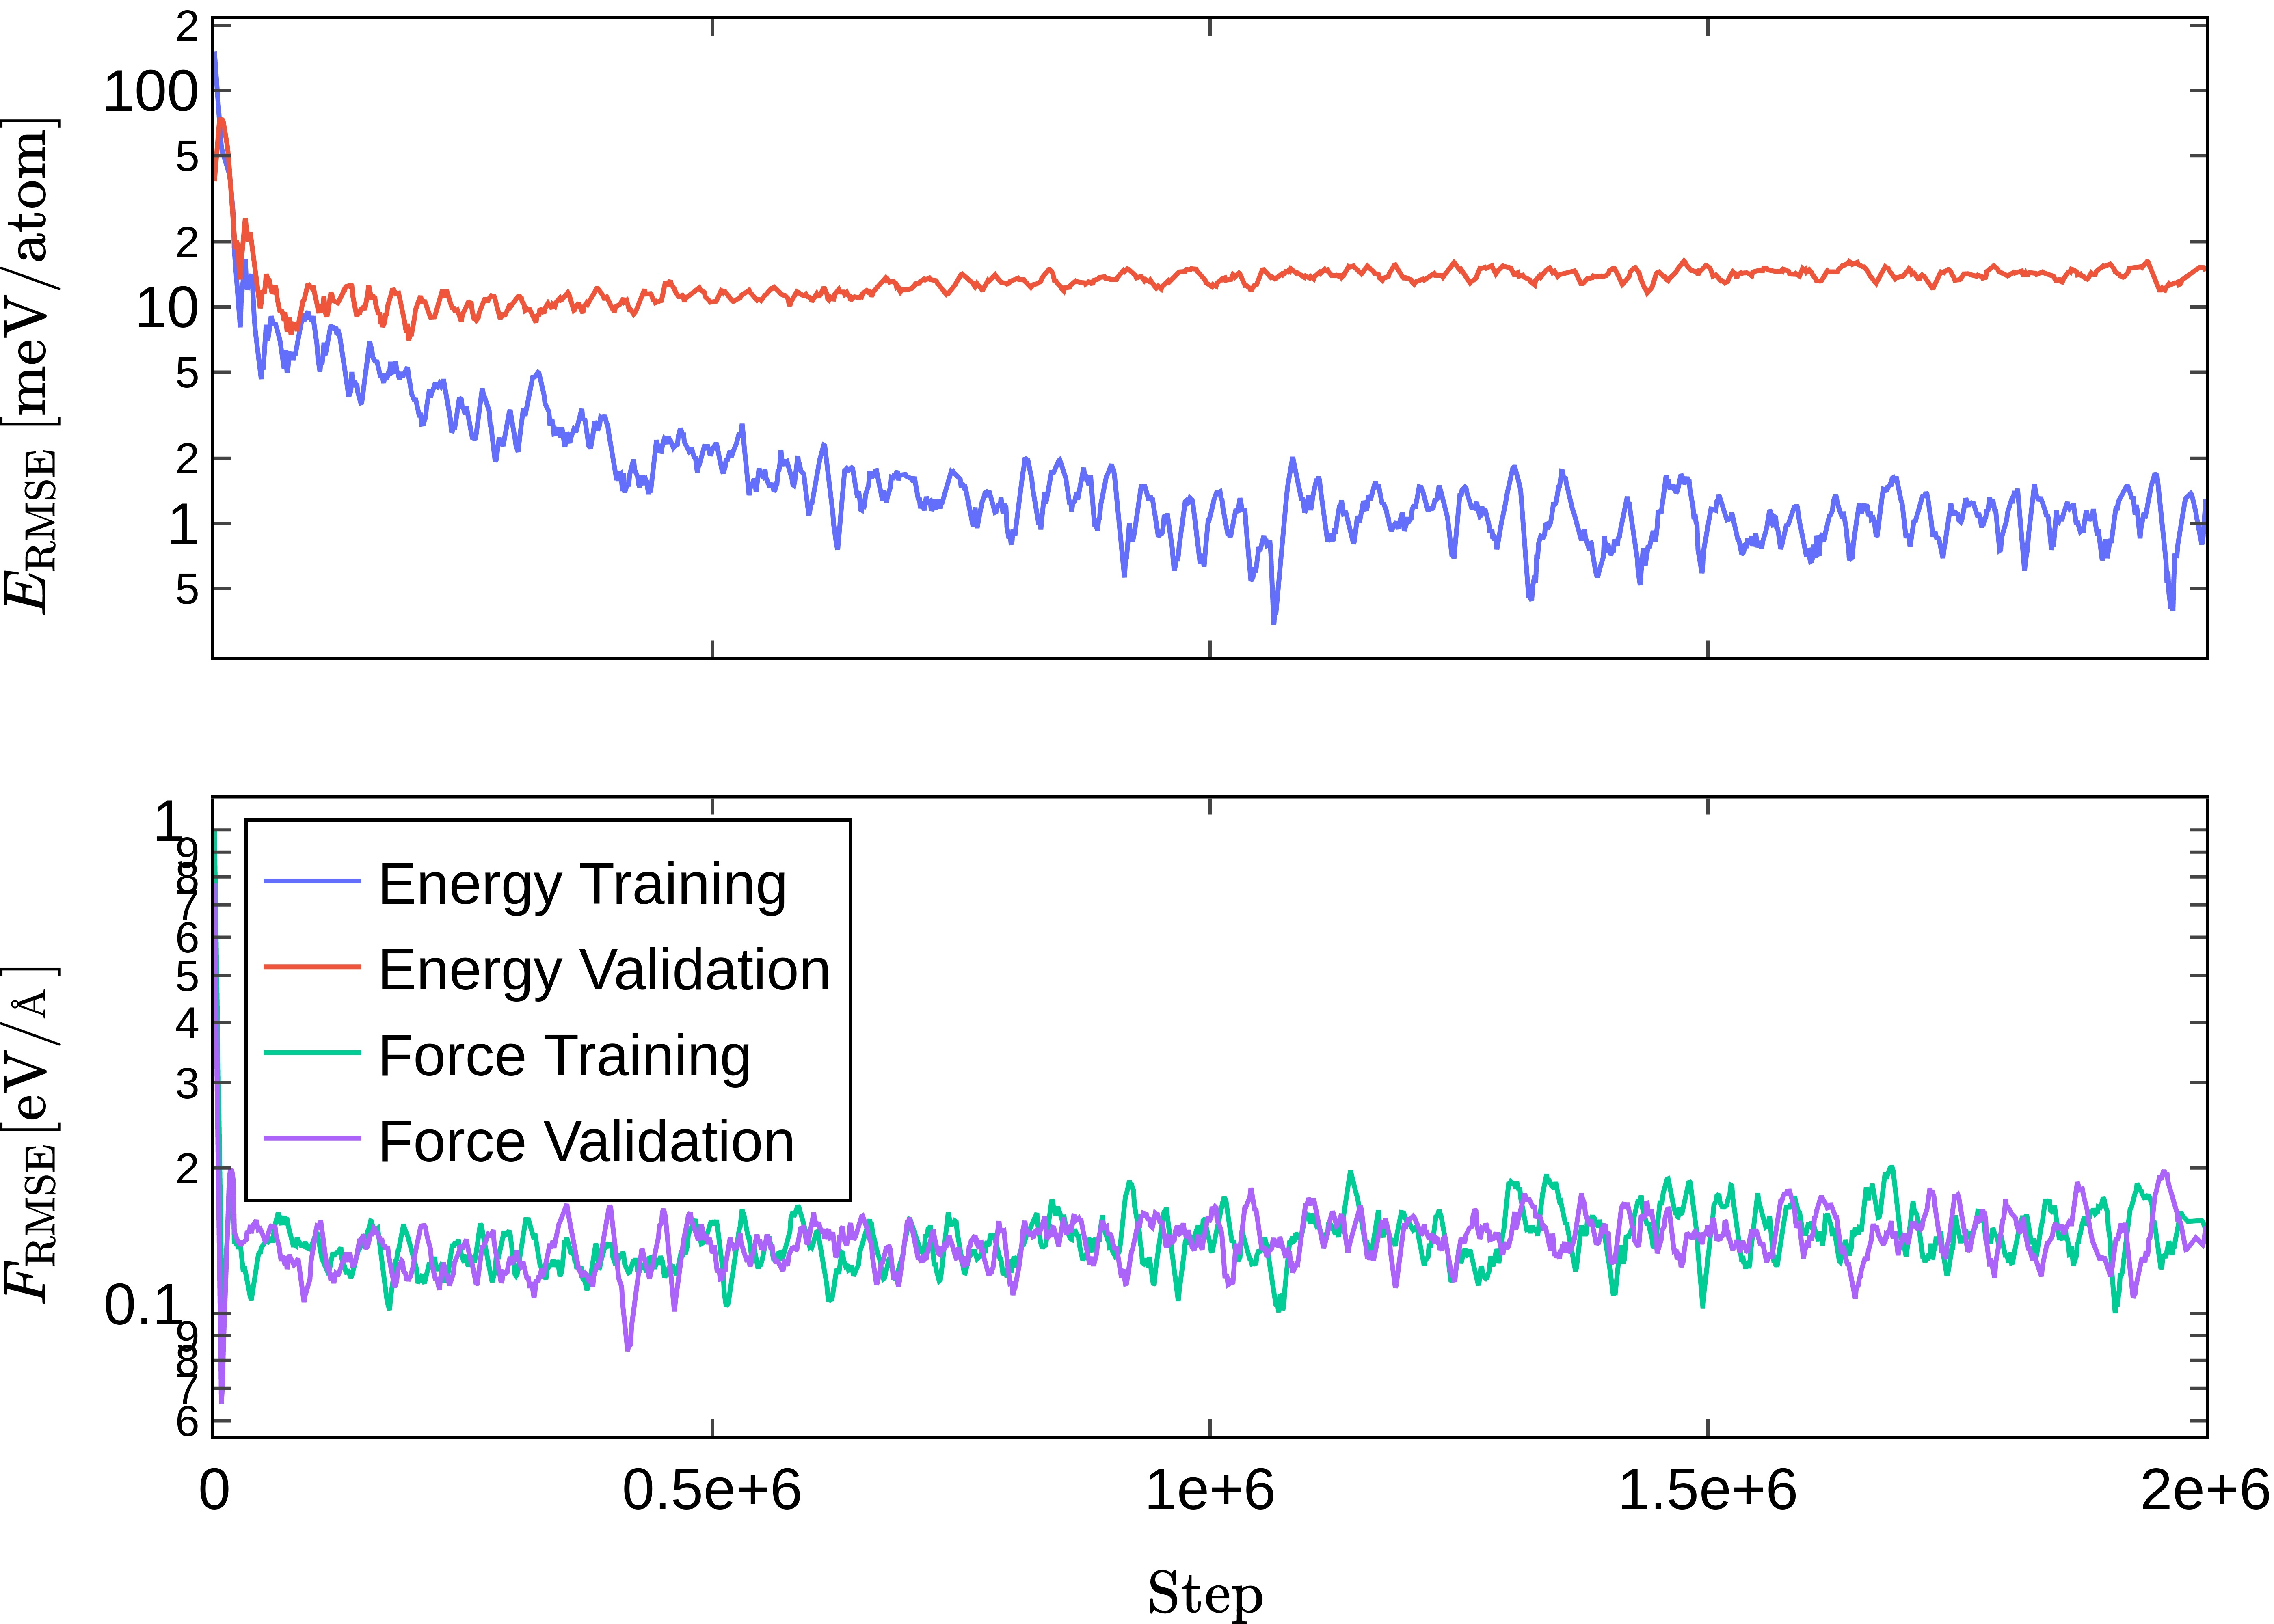
\includegraphics[width=.8\textwidth]{
      asset/crystalline_10,20,40d_75,75,75f_260222622s_energy_force_l_curve.jpg
    }
  \end{center}
  \caption{Learning curves for model \texttt{crystalline\_10,20,40d\_75,75,75f\_260222622s}.}
  \label{fig:crystalline_10,20,40d_75,75,75f_260222622s-learning-curves}
\end{figure}

\begin{figure}
  \begin{center}
    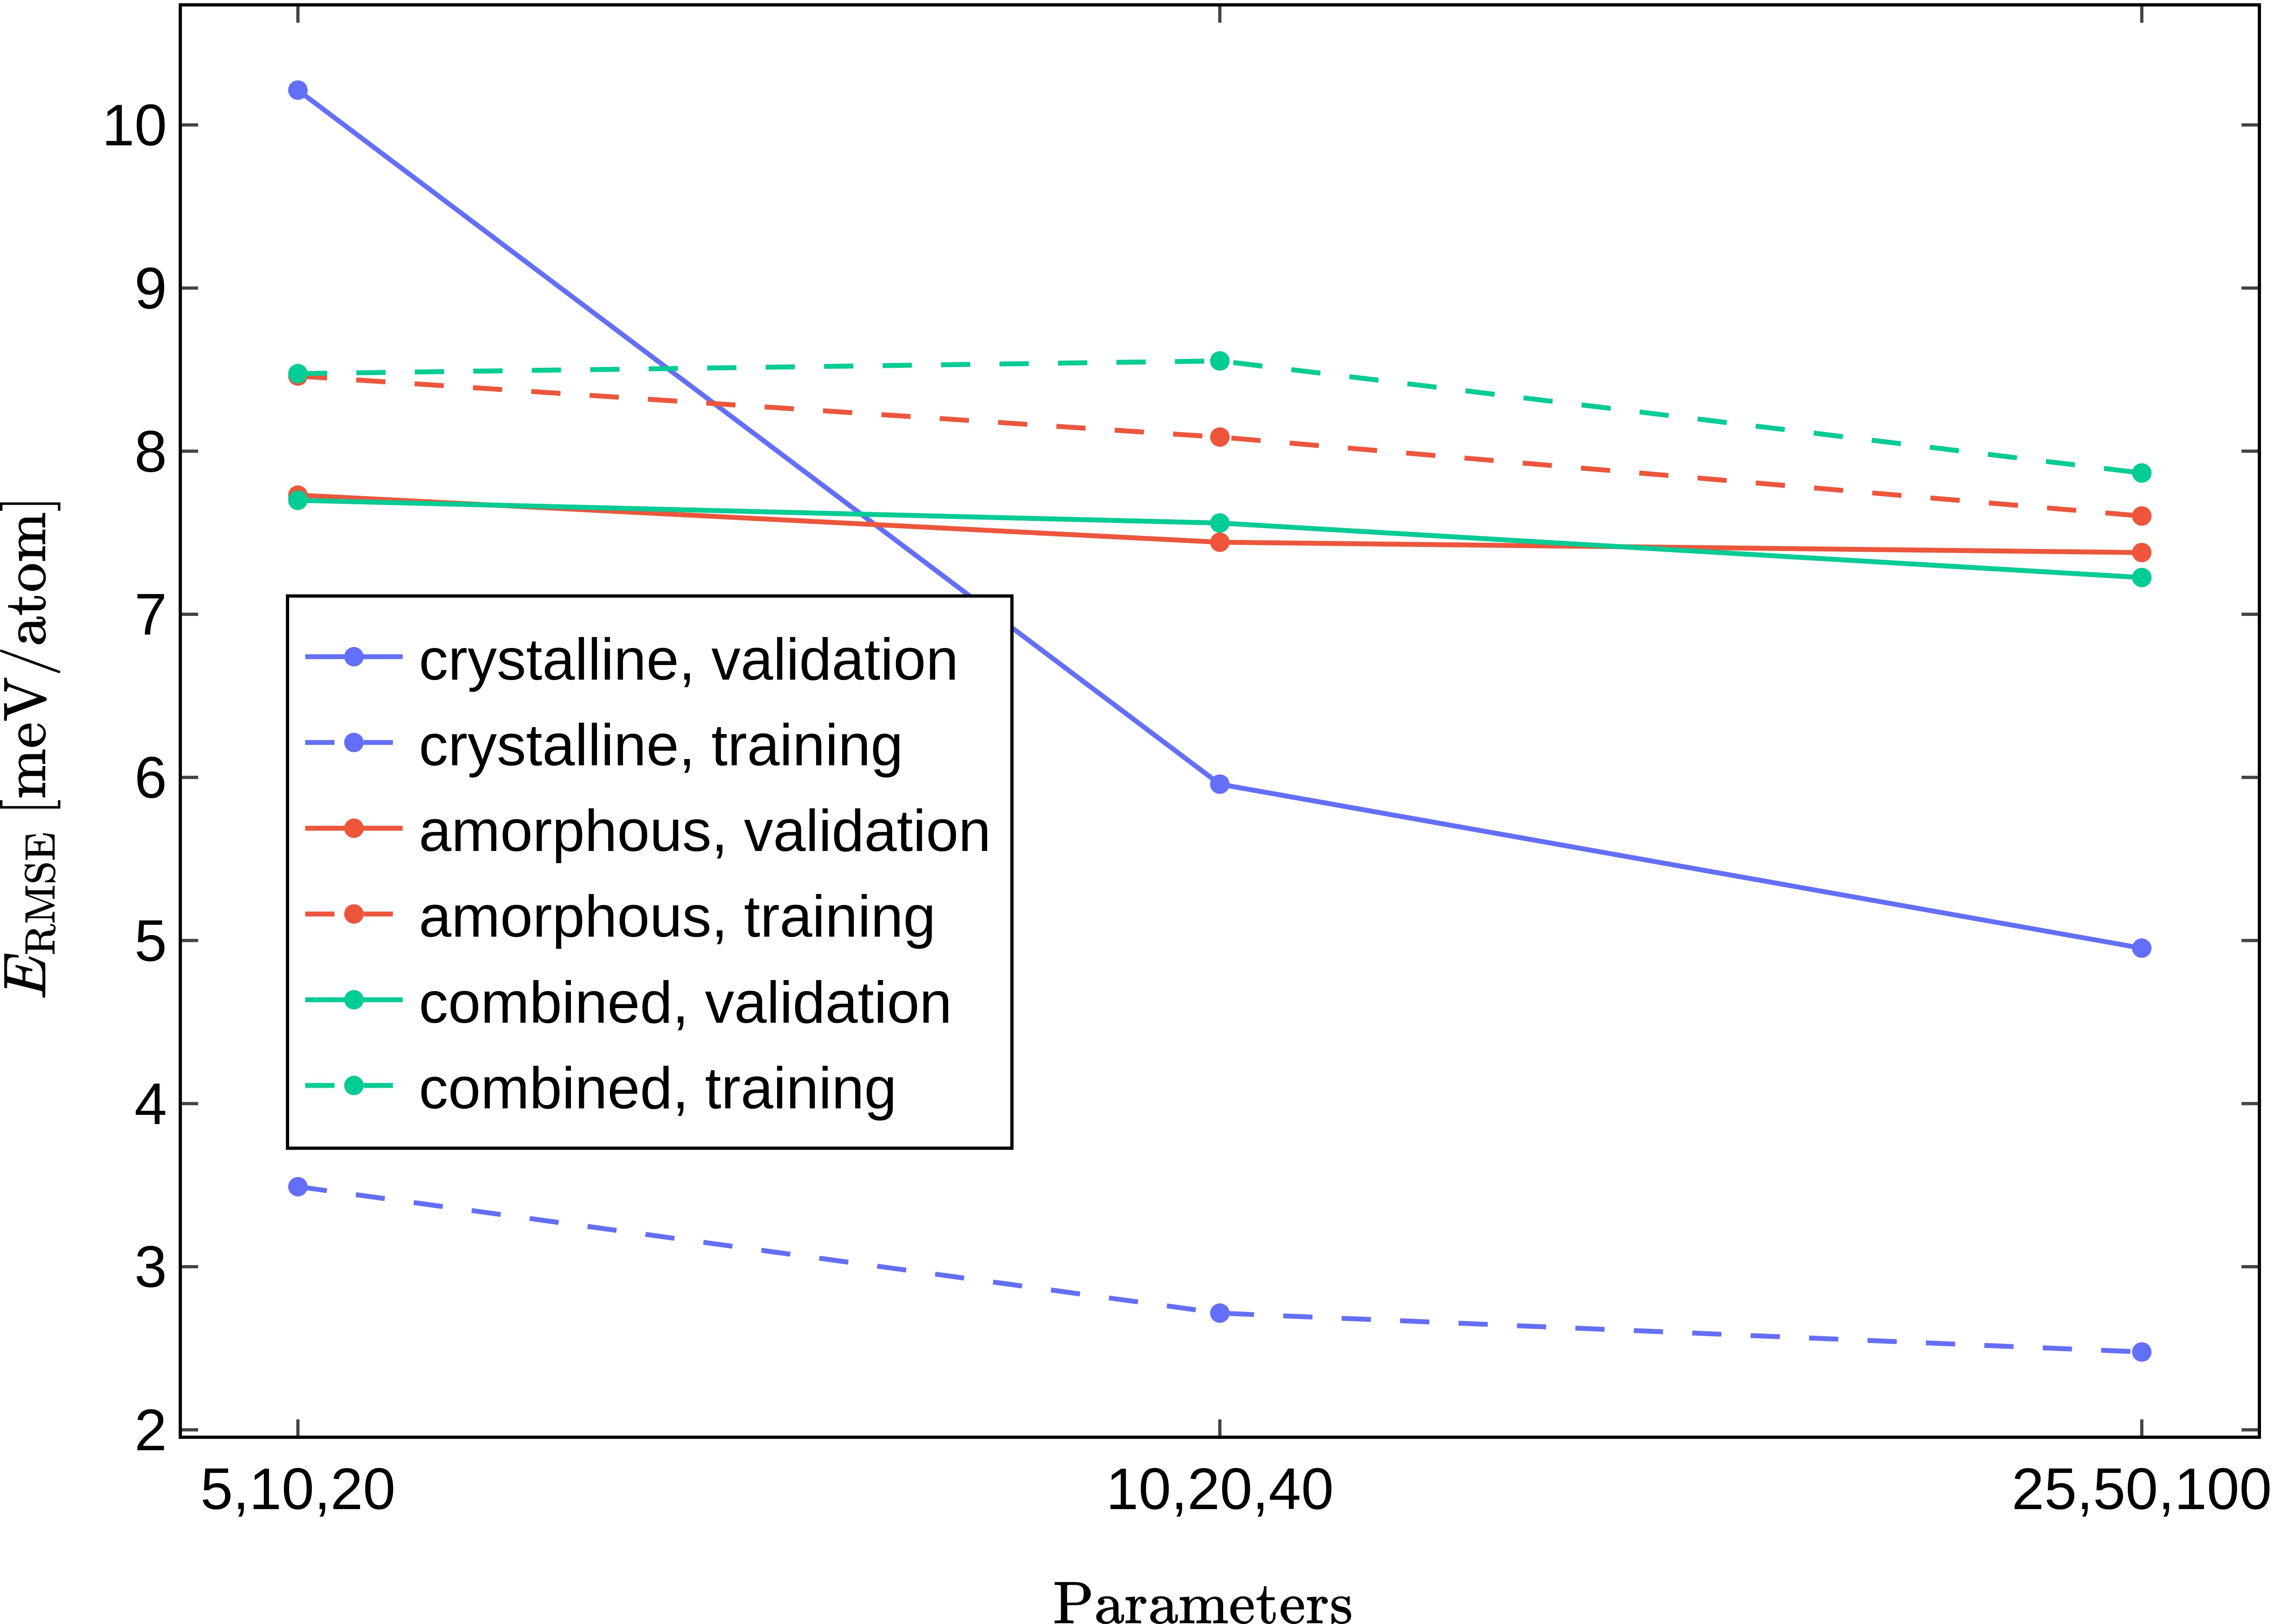
\includegraphics[width=.8\textwidth]{
      asset/descriptor_energy_error_evaluation.jpg
    }
  \end{center}
  \caption{Evaluation of energy errors for different descriptor neuron numbers.}
  \label{fig:descriptor_energy_error_evaluation}
\end{figure}

\begin{figure}
  \begin{center}
    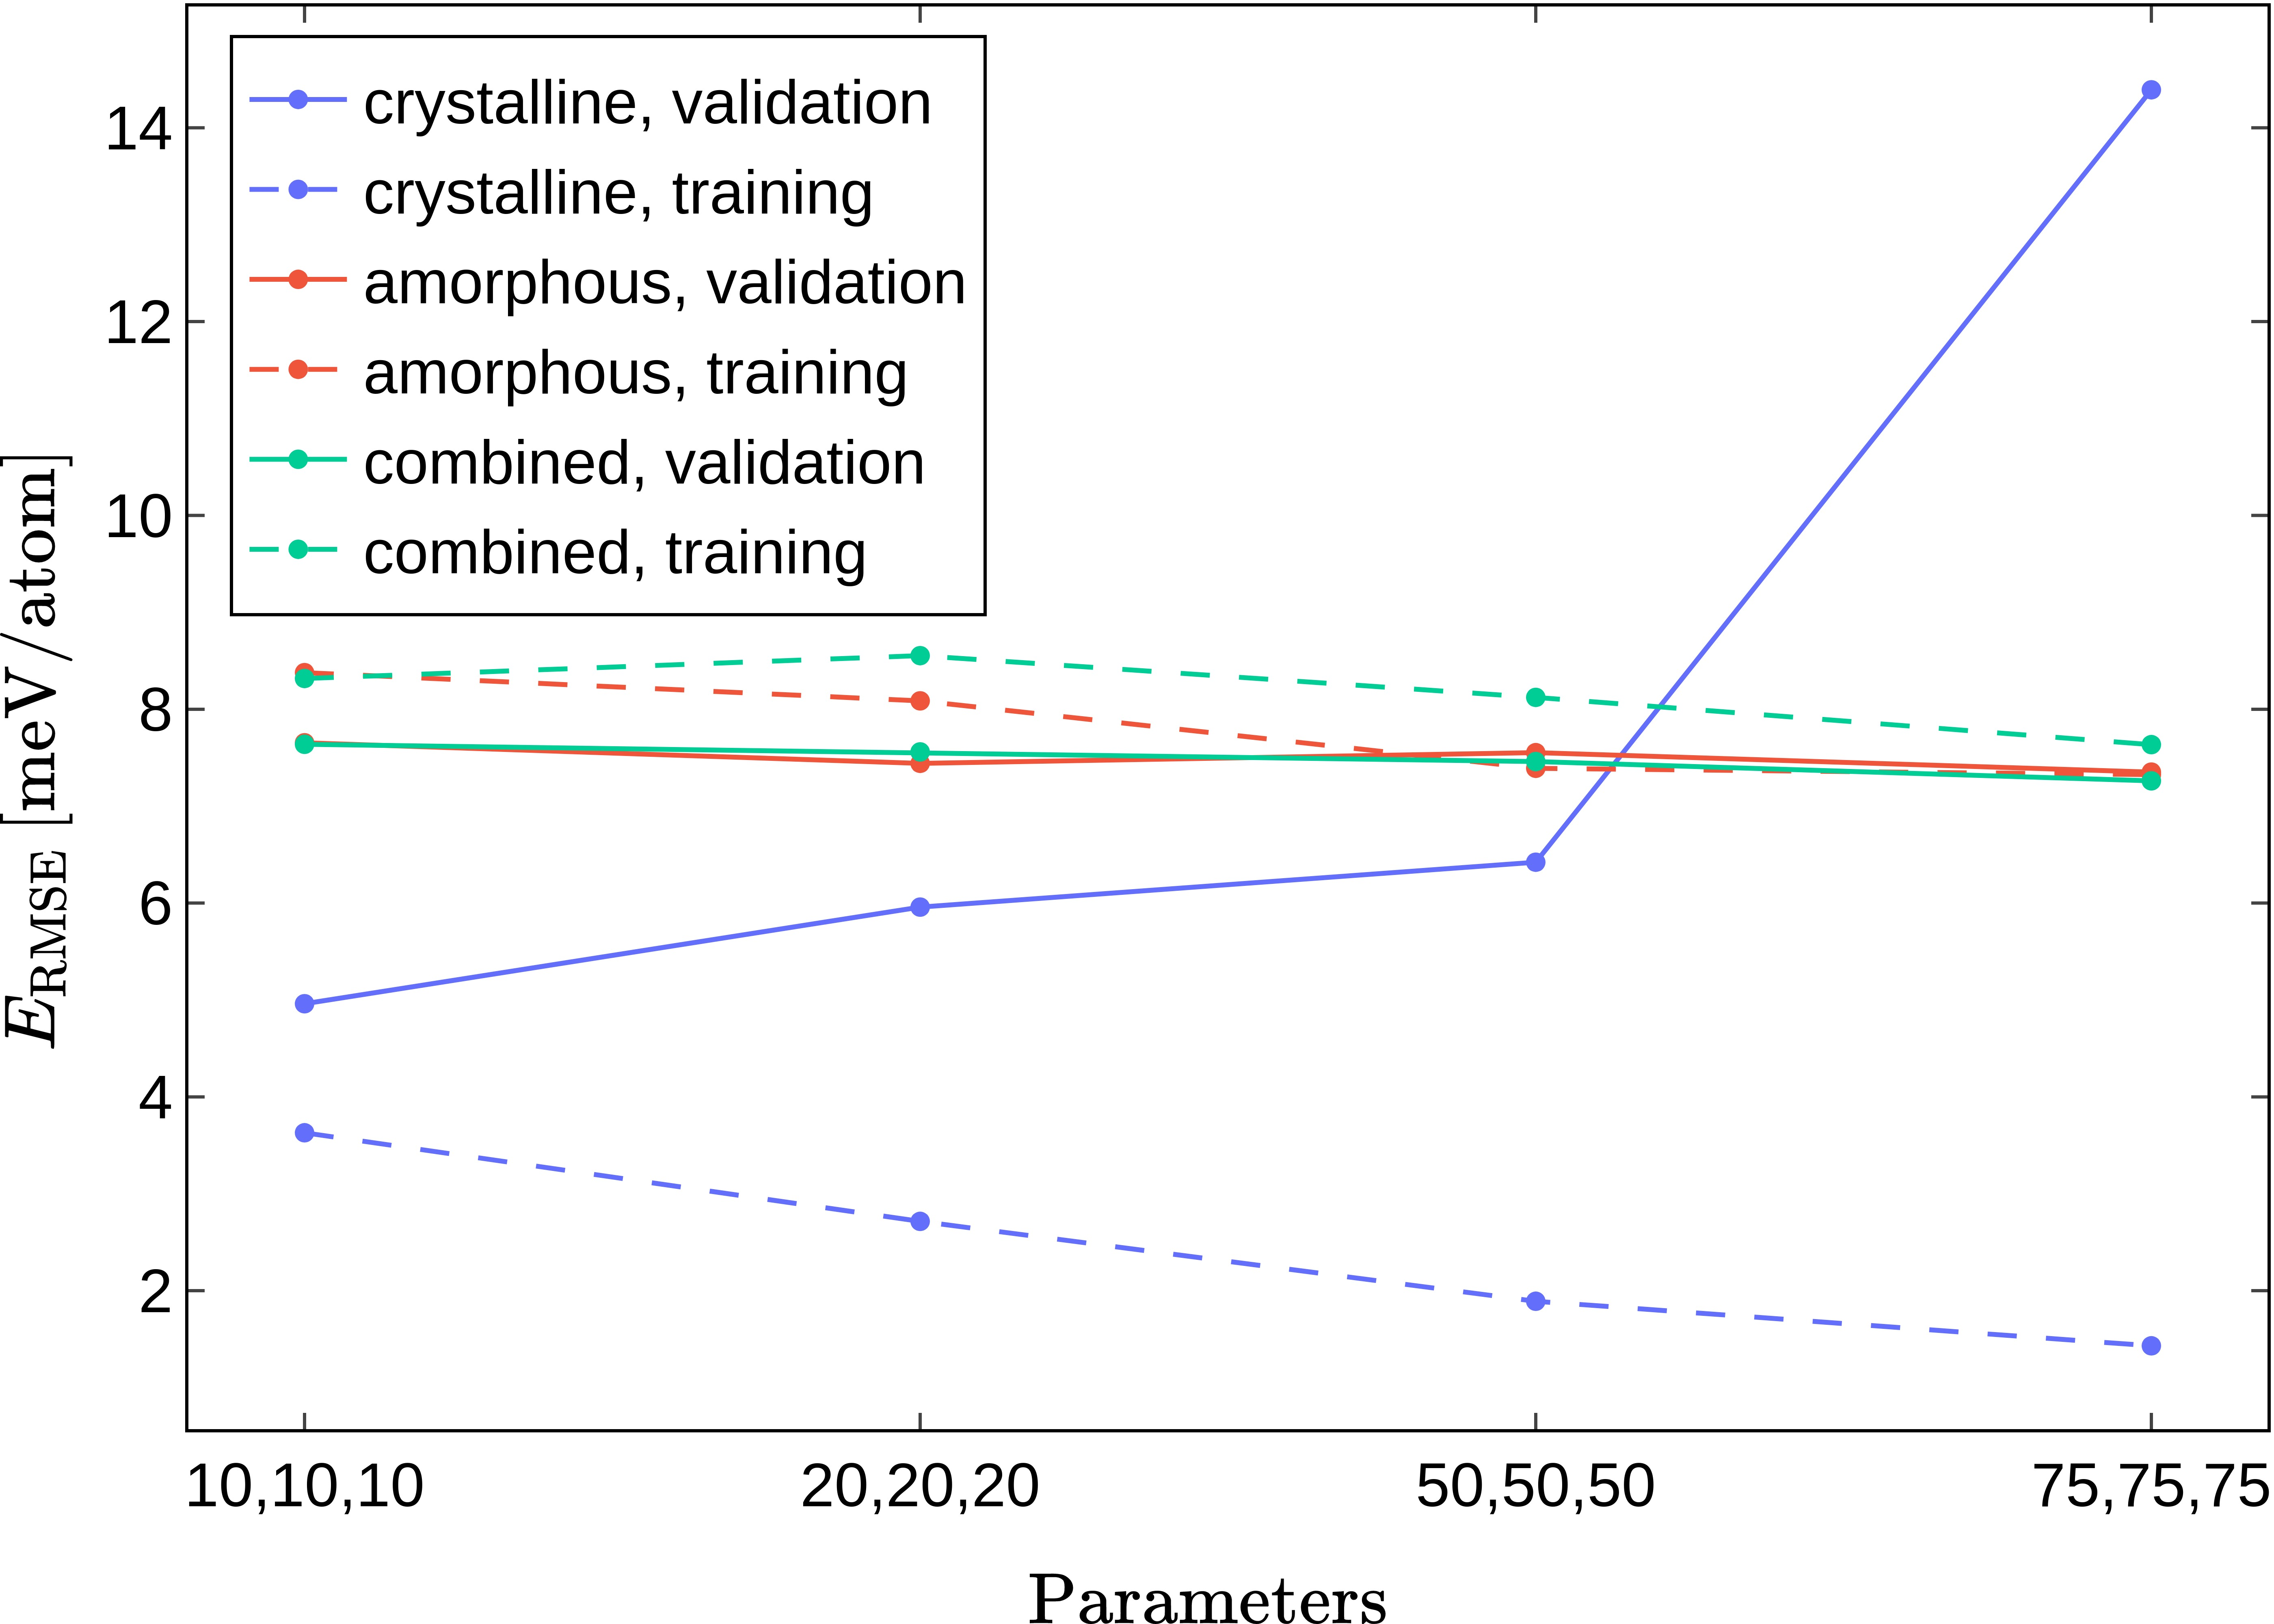
\includegraphics[width=.8\textwidth]{
      asset/fitting_energy_error_evaluation.jpg
    }
  \end{center}
  \caption{Evaluation of energy errors for different fitting neuron numbers.}
  \label{fig:fitting_energy_error_evaluation}
\end{figure}

\section{Inference Results}
